\documentclass[12pt] {article}
\usepackage[margin=1in]{geometry} %one inch margins
\renewcommand{\baselinestretch}{1.5} %double space, safe for fancy headers
\usepackage{pslatex} %Times font
\usepackage{graphicx} %for figures
\usepackage{enumerate} %for lists
\usepackage{fancyhdr} %header
\pagestyle{fancy}
\usepackage[font={small,sf},format=plain,labelfont=bf,up]{caption}
\fancyhf{}
\fancyhead[l,lo]{150001C \textit{ Internship Report}} %left top header
\fancyhead[r,ro]{\thepage} %right top header
\usepackage{kernelstyle}
\usepackage{listings}
\usepackage{amsmath,amssymb,amsfonts,amsthm}
\usepackage{graphicx}
% \usepackage[utf8]{inputenc}
\usepackage{float} 
\usepackage[caption=false,font=timesnewroman]{subfig}
\usepackage[final]{pdfpages}
\usepackage{gensymb}

\graphicspath{{figures/}}

\usepackage{xcolor}
\usepackage{soul}
\usepackage{hyperref}
\hypersetup{
    colorlinks=true,
    linkcolor=blue,
    filecolor=magenta,      
    urlcolor=cyan,
}
\captionsetup[figure]{labelfont={bf},name={Fig.},labelsep=period}
\captionsetup[table]{labelfont={bf},name={Table.},labelsep=period}
\usepackage{caption}
\usepackage{chngcntr} 
\counterwithin{figure}{section}
\counterwithin{table}{section}


\usepackage{algorithmic}
\usepackage[ruled, noend,lined,linesnumbered]{algorithm2e}

\newcommand{\hlc}[2][yellow]{{%
    \colorlet{foo}{#1}%
    \sethlcolor{foo}\hl{#2}}%
}

\usepackage{hyperref}
\hypersetup{
   colorlinks=true,
   linkcolor = black,
   citecolor=Green
}


\title{INTERNSHIP REPORT}


\definecolor{hgray}{RGB}{130,130,130}
\definecolor{hred}{RGB}{136,0,0}
\definecolor{black}{RGB}{0,0,0}
\definecolor{Green}{RGB}{0,255,0}

\usepackage[T1]{fontenc}
\usepackage[tableposition=top]{caption}
\usepackage{rotating}
\usepackage{color, colortbl}
\usepackage{booktabs, array, dcolumn}
\usepackage{tikz}
\usepackage{graphicx}
\usepackage{pgf-umlsd}
\usepackage{multirow}
\usepackage{epsfig}
\usepackage{subfig}
\usepackage{pgfplotstable}
\usepackage{amsfonts}
\usepackage{relsize}
\usepackage{varwidth}
\usepackage{url}
\usepackage{amsmath}
\usepackage{amssymb}
\usepackage{booktabs}
% \usepackage{soul}
\usepackage[normalem]{ulem}
\usepackage{subfig}
\usepackage{kernelstyle}
\definecolor{Gray}{gray}{0.9}
\usepackage{hyperref}
% \usepackage{tabularx}
\usepackage{footnote}

\definecolor{gray1}{gray}{0.9}
\definecolor{gray2}{gray}{0.6}
\definecolor{Gray}{gray}{0.9}


\definecolor{light-gray1}{gray}{0.65}
\definecolor{light-gray2}{gray}{0.95}

%%------------------------ PREAMBLE ENDS ---------------------------

\begin{document}
\pagenumbering{roman} % Start roman numbering


\newpage

\tableofcontents
\newpage
\listoffigures
\listoftables
\newpage
\pagenumbering{arabic}
%!TEX root = ./intern_report.tex
\section*{Preface}

\paragraph{}
Described in this report is the 24 week training experience I had in wave computing/Paraqum Technologies dating from 25.06.2018 to 07.12.2018 for the fulfillment of industrial training requirements of my B.Sc. in Electronics and Telecommunication Engineering. The report consists of 3 main sections as follows

\subsubsection*{Chapter 1: Introduction to Wave computing and Paraqum Technologies}
\paragraph{}
Wave computing is a USA based AI startup and Paraqum Technologies is a Sri Lankan Electronic design startup. Wave is now ranked among the top 25 AI providers of the world~\cite{top25ai} and Paraqum Technologies is highly respected in Sri Lanka as a pioneer of the industry and recieves design contracts from all over the world. Our training was done through a design contract offered to Paraqum by Wave computing.

\subsubsection*{Chapter 2: Training Experience}
\paragraph{}
Even though I was an intern, I was given full exposure to the company workflow. I recieved a full scale project to lead and a support team from all over the world to work with. Everyone in the company were very supportive and friendly. The environment was comfortable to work and the workload was perfectly balanced, demanding yet not overwhelming.

\subsubsection*{Chapter 3: Conclusion}
\paragraph{}
I can say without a doubt, this is one of the best training experiences one can get. The University of Moratuwa Industrial training division, the Department of Electronic and Telecommunication Engineering and National Apprentice and Industrial Training Authority (NAITA) together did their best to provide us with an exceptional experience that will be very useful for the future of our careers.

\newpage
\section*{Acknowledgment}

\paragraph{}
I take this chance to show my gratitude towards everyone that helped make this training possible and facilitated my time with it. First of all I should thank the industrial training division of University of Moratuwa and the National Apprentice and Industrial Training Authority (NAITA) for allowing us to get an industrial training of this magnitude and quality during the time of our studies and always looking out for the wellbeing of the trainees.

\paragraph{}
I also would like to thank the administration and staff of Paraqum Technologies, starting with the CEO Dr. Ajith Pasqual, Manager Eng. Hasanka Sandujith, Eng. Kasun Tharaka who coordinated the internships and all other staff members who helped in a great many ways to make the training a staggering success. 

\paragraph{}
Last but definitely not least, The staff of the Wave computing team (later separated as Wave computing Sri Lanka) were always dedicated to make the training worthwhile for us. I sincerely thank the Senior Director of Software Engineering division of wave computing Eng. Henrik Esbenson, who visited and supervised us from time to time, General manager of Wave computing Eng. Nuwan Gajaweera, Technical leaders Eng. Upul Ekanayaka and Eng. Binu Amarathunga, My supervisors Eng. Achintha Ihalage, Eng. Omega Gamage and SDK team lead Eng. Dakila Serasinghe and all other staff members of wave computing for everything they did for us.

\vspace*{3cm}

\noindent Chinthana Wimalasuriya,\newline
Undergraduate,\newline
Department of Electronics and Telecommunication Engineering,\newline
University of Moratuwa.

\newpage
\section{Introduction to the Training Establishment}
%!TEX root = ./intern_report.tex

\subsection{Company Overview}
\subsection{Company History}
\subsection{Organization Structure and Hierarchy}
\subsection{Areas of Interest}
\subsection{Current Situation}
\subsection{Impacts on Sri Lankan Industry}

\subsection{SWOT Analysis}
\subsubsection{Strengths}
\subsubsection{Weaknesses}
\subsubsection{Opportunities}
\subsubsection{Threats}

\subsection{Usefulness to the Country}
\subsection{Suggestions to Improve the Company}

\newpage
\section{Training Experience}
%!TEX root = ./intern_report.tex

\subsection{How I got the Opportunity}

\paragraph{}
A long time before the industrial training selection, I had heard Paraqum Technologies was one of the best places to learn about the electronics industry in Sri Lanka and Its CEO, Dr. Ajith Pasqual had taught a module in the university that sparked an interest in me about the subject of silicon design. Therefore, when Paraqum Technologies was listed as an open CV company, I did not hesitate to submit a CV, which got selected by the company staff who then interviewed me thoroughly in their office and sometime later, informed me that I had been selected to the Wave Computing Division.

\paragraph{}
At the start of the Internship, I was placed under the supervision of Eng. Achintha Ihalage, an application engineer whose original task was to handle the timing and constraints of the DPU chip. He walked me through the basics of setting up the Wave Computing workspace, company work ethics and other needed technical skills. He also introduced us to the DPU hardware and other proprietary technologies by Wave. 

\paragraph{}
During the second week, Eng. Henrik Esbenson, who is in charge of the Sri Lankan team at Wave HQ visited the office and demonstrated his ideas for projects. One of these was the Python - Wave Flow Graph translator, also known as Py2WFG. I volunteered to take that project and Eng. Henrik allocated me the necessary resources of the company including support teams and software tools to carry on the project.

\paragraph{}
This project soon became popular among the crowd of wave computing and I developed it according to the requirements and feedback. The amount of work was rather large but I managed to complete the project and hand it over by the time Internship ended. This project will most likely be adopted by full time developers and expanded to probably replace the existing design flow.


%!TEX root = ./intern_report.tex

\newpage
\subsection{Trailnet: A Classification Network for Autonomous Trail Navigation}

\subsubsection{Trailnet: An Introduction}

\begin{figure}[H]
    \centering
    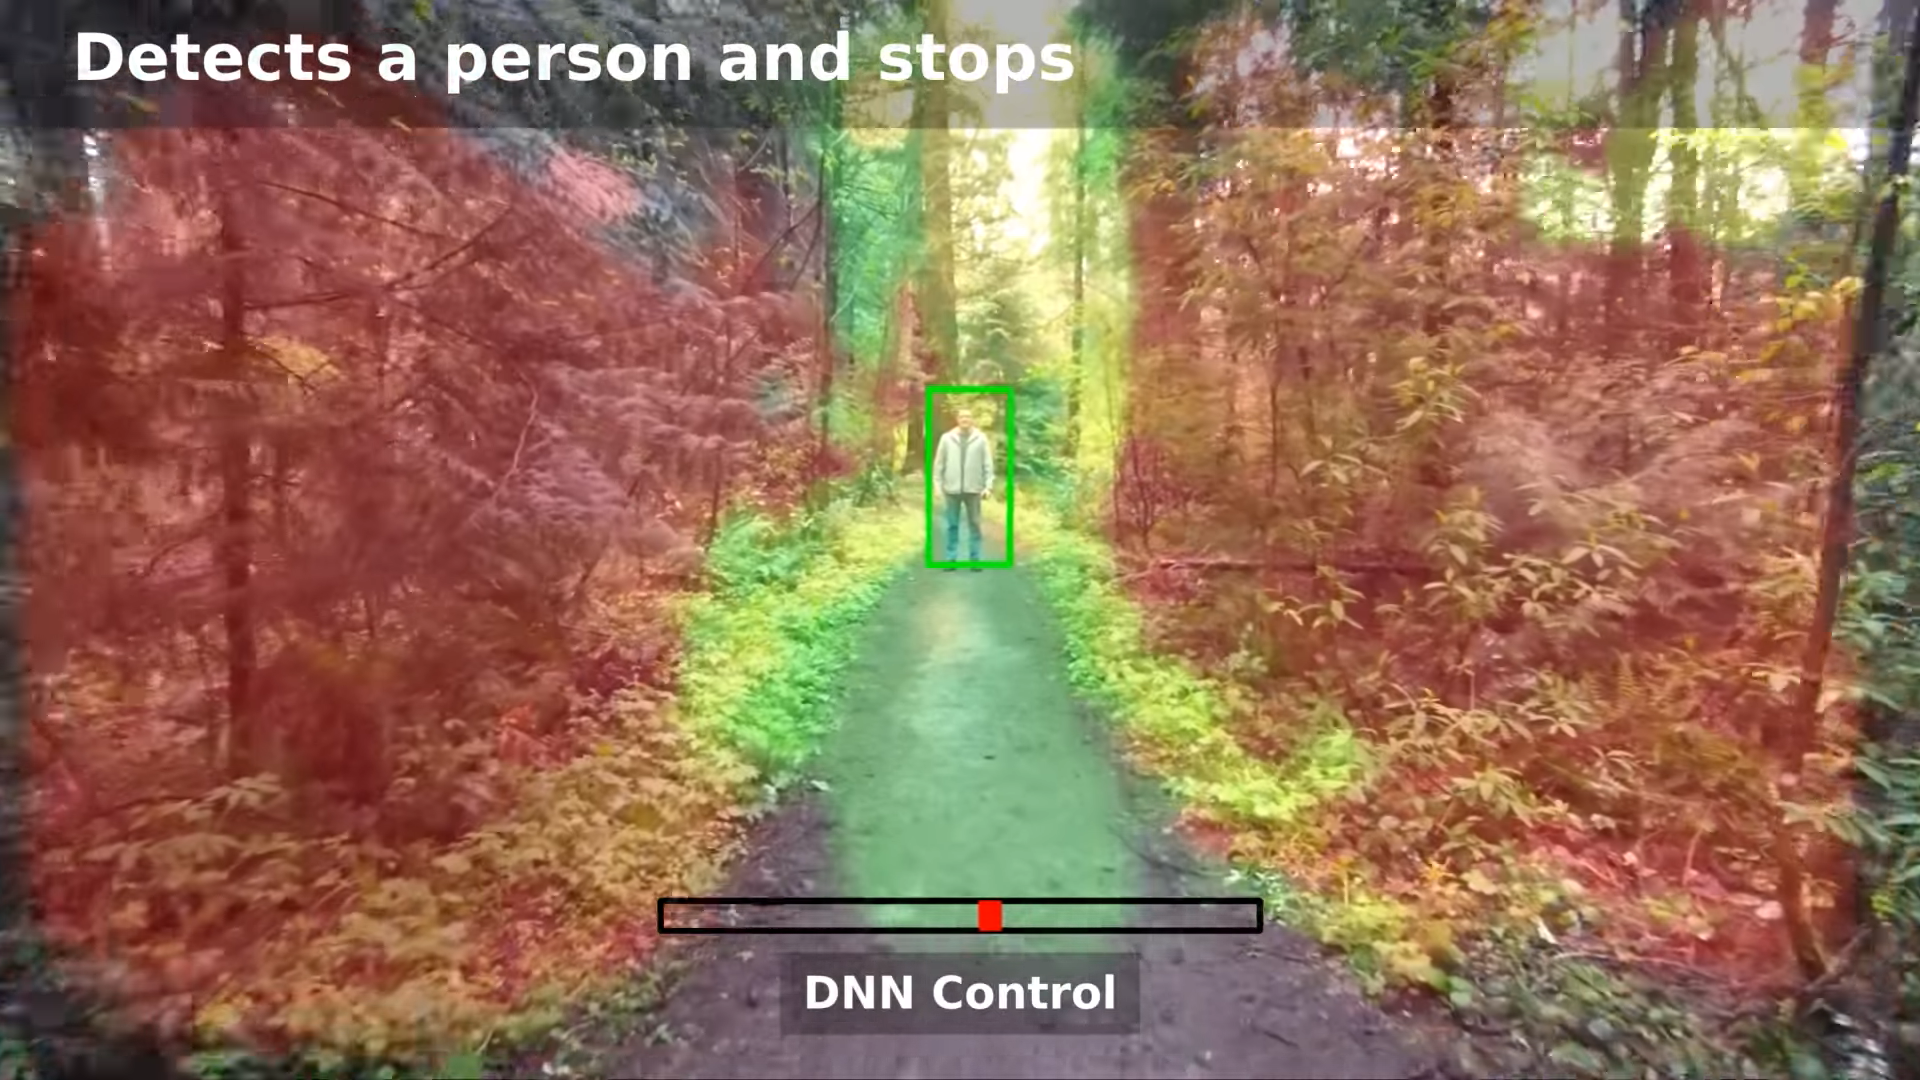
\includegraphics
        [width=10cm]
        {figures/trailnet_redtail_object.png}
    \caption{NVIDIA's Trailnet Navigating a Drone}\vspace{-4mm}
\end{figure}

In 2017, four researchers published a paper titled "Toward Low-Flying Autonomous MAV Trail Navigation using Deep Neural Networks for Environmental Awareness" ~\cite{trailnet} (Trailnet paper in short) with the funding of NVIDIA. The paper describes the following:

\begin{itemize}
    \item Merits of approaching autonomous navigation as a classification problem
    \item Architecture of their Trailnet CNN, a modified version of Resnet-18. ~\cite{resnet}
    \item Data collection techniques for the Trailnet CNN
    \item Training Trailnet with a relatively small dataset
    \item Hardware hierarchy and the command flow between cameras, NVIDIA Jetson TX2 ~\cite{jetson_tx2} running ROS and the flight control board.
    \item Usage of YOLO ~\cite{yolo} for obstacle detection and algorithm for obstacle avoidance.
    \item Results and observations after flying the quadcopter autonomously in the forest trail for several kilometers.
\end{itemize}

\newpage
\subsubsection{Navigation as Classification} 

\paragraph{}
Their model was based on a concept discussed in a 2016 paper ~\cite{trailnet},
: approaching autonomous navigation as a classification problem. That is, given an RGB image the CNN would output three probabilities: that of the camera facing left, right or center with respect to the trail. The key advantages in this approach are:

\begin{itemize}
    \item The effect of noise introduced by human errors during data collection on training are minimized due to discretization.
    \item Data collection and labeling is straightforward
    \item Performance can be fine tuned, by adjusting K1 and K2 accordingly. See Figure: \ref{Fig:trailnet_archi}
    \item The depth of the required neural network is less, compared to the regression network that provides similar accurate performance.
    \item Can train the relatively shallow network with a relatively small dataset and shorter training time.
    \item Can be implemented on low powered devices.
\end{itemize}

In the Trailnet paper ~\cite{trailnet}, they choose Resnet 18 as the basis for their architecture since it is small enough to be run on real time in a power-limited device like Jetson TX2. Resnets (Residual Networks) are special kinds of deep neural network that uses "short circuits" between layer outputs to prevent the problem of vanishing gradients, as a network gets too deep. By employing this technique, researchers have been able to create networks that are thousands of layers deep and still outperform shallower networks. Resnet-18, Resnet-50...etc are popular variants of applying this technique on deep convolutional neural networks.

\paragraph{}
Trailnet is not an RCNN. That is, it does not remember past inputs nor correlate current inputs with past and future values for prediction. It is a simple CNN that gives a twist command based on the current image. Input to trailnet is a 320 x 180 x 3 RGB image and the outputs are six softmax nodes connected to the output of a slightly modified resnet-18. The six output layers signify the probability of the given image facing left, center and right and the robot (or UAV) being aligned left, center and right on the path. Weighted (by adjustable constants k1, k2) sum of these probabilities provide the angular twist command, which is used to steer the robot. This additional consideration of alignment, prevents the UAV slowly drifting off the center of the trail and crashing with tree branches near the trail edges. Together, the facing and align probabilities correct the course of the UAV to stay in the center of the path. YOLO ~\cite{yolo} and SLAM are used for obstacle avoidance.

\paragraph{}
Data collection was done using a camera rig with 3 cameras facing at three angles (left, center and right). The rig was carried by a person along a forest trail. The video feed from each camera had been then labeled accordingly. Similarly align to left, center and right data has been collected. A pretrained network (previously trained on IDSIA dataset ~\cite{idsia} of 40,000 images) had been fined tuned with this collected data. After training, Trailnet was run with ROS (Robot Operating System) and Caffe on Jetson TX2 on board the UAV. Jetson TX2 receives the video frame from camera, processes it and sends it sends command to the flight controller. This was further improved by other researchers around the world ~\cite{trailnet2}, ~\cite{trailnet3}, ~\cite{trailnet4}.



\subsubsection{Building Trailnet from scratch}

\paragraph{}
One objective of their project was to showcase the capability of NVIDIA's Jetson TX2 high level controller board. Therefore, they had used Caffe framework to build the network and DIGITS framework to train it. However, our key objective in working with this was to build a unified pipeline which all scientists in DATA61 can use. Since most of them were familiar with TensorFlow and since it is the state of the art framework today, I rebuilt the 20-layer network in TensorFlow-Keras and trained it from scratch in CSIRO's supercomputer as I built the pipeline.

% Image: Architecture
\begin{figure}[H]
    \centering
    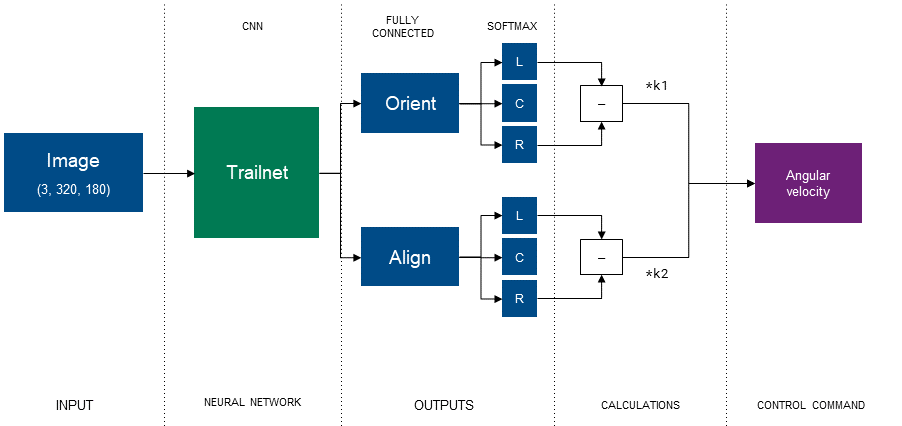
\includegraphics
        [width=16cm]
        {figures/trailnet.PNG}
    \caption{Simplified Trailnet Architecture and Post Processing}\vspace{-4mm}
    \label{Fig:trailnet_archi}
\end{figure}

\subsubsection{Data collection and training Trailnet from scratch}

\paragraph{}
Our goal with this project was to train a robot navigate indoor hallways as a demonstration of our end-to-end pipeline. Hence we mounted three cameras on the robot, facing center, left and right by 30 degrees. We took the robot along the hallways of CSIRO using a remote control and recorded the image stream data as ROS bags. In each hallway, we took the robot on three paths: center aligned, left aligned and right aligned. We then extracted the image stream into an image dataset by taking one image every second (1 fps) from the image stream. The resulting hallway dataset consisted of 120,000 images.

% Image: IDSIA
\begin{figure}[H]
    \centering
    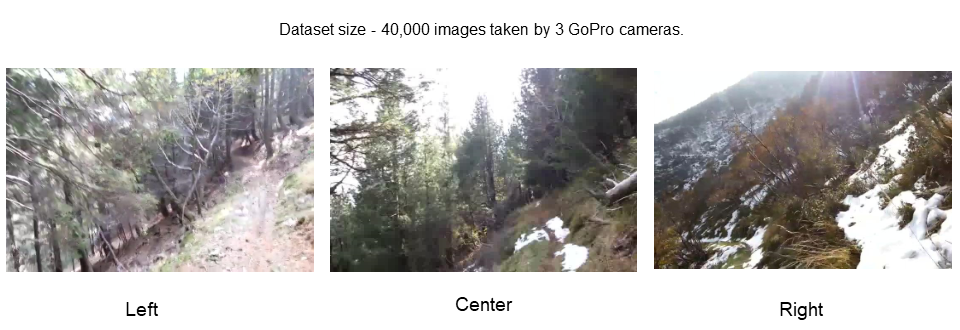
\includegraphics
        [width=16cm]
        {figures/idsia_dataset.PNG}
    \caption{IDSIA Dataset of 40,000 images}\vspace{-4mm}
\end{figure}

% Image: Hallway Dataset
\begin{figure}[H]
    \centering
    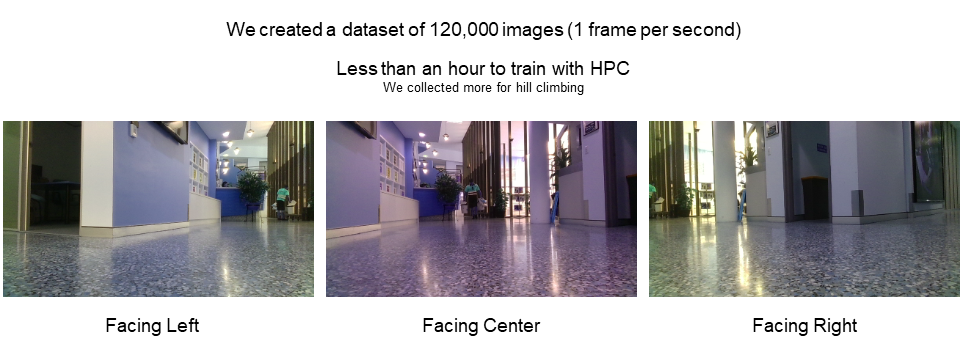
\includegraphics
        [width=16cm]
        {figures/hallway_dataset.PNG}
    \caption{Hallway Dataset of 120,000 images}\vspace{-4mm}
\end{figure}


\paragraph{}
The 120,000 images were stored in the supercomputer and used to train the network. First, align output nodes of Trailnet were frozen and the network (with facing output nodes only) was trained on the IDSIA dataset ~\cite{idsia}
 of 40,000 images. Then, the same configuration was trained on the hallway facing dataset. Finally, the facing-output nodes were frozen and the rest (align-output nodes) were trained on the hallway-align dataset.

\paragraph{}
Training the network was a laborious process prone to errors. The supercomputer sessions automatically terminate every few hours, requiring me to stay by the CSIRO provided desktop throughout the process. I stayed overnight for five days alone in the office to train this and the other networks.

\subsubsection{Deployment on a Robot and Testing}

\paragraph{}
The trained model was optimized into a tf-trt graph (See section: \ref{tensorrt}) and executed inside a python based ROS node. The latency was 20 ms, which was enough to process an input image stream at 30 fps during inference. My ROS node also performs necessary calculations and publishes a velocity message (type: geometry\_msgs/Twist)  to a topic that is subscribed by the motor controller and the predictions (type: Float32MultiArray) for debugging. I also designed it in a way that the constants K1, K2 can be tuned by publishing the constants to a topic that is subscribed by the Trailnet ROS node.

\paragraph{}
After setting up this way, the robot was tested for its ability to navigate the hallways autonomously. It's response to external disturbances was checked by kicking the robot in either direction, moving it off the center of the track. K1, K2 constants were tuned to provide the shortest response time while maintaining a steady speed when undisturbed. We also created a visualization technique, where the predictions and commands of the robot can be visualized with the image stream. Following images show the testing process and the corresponding visualization.

% Image: Disturbances
\begin{figure}[H]
    \centering
    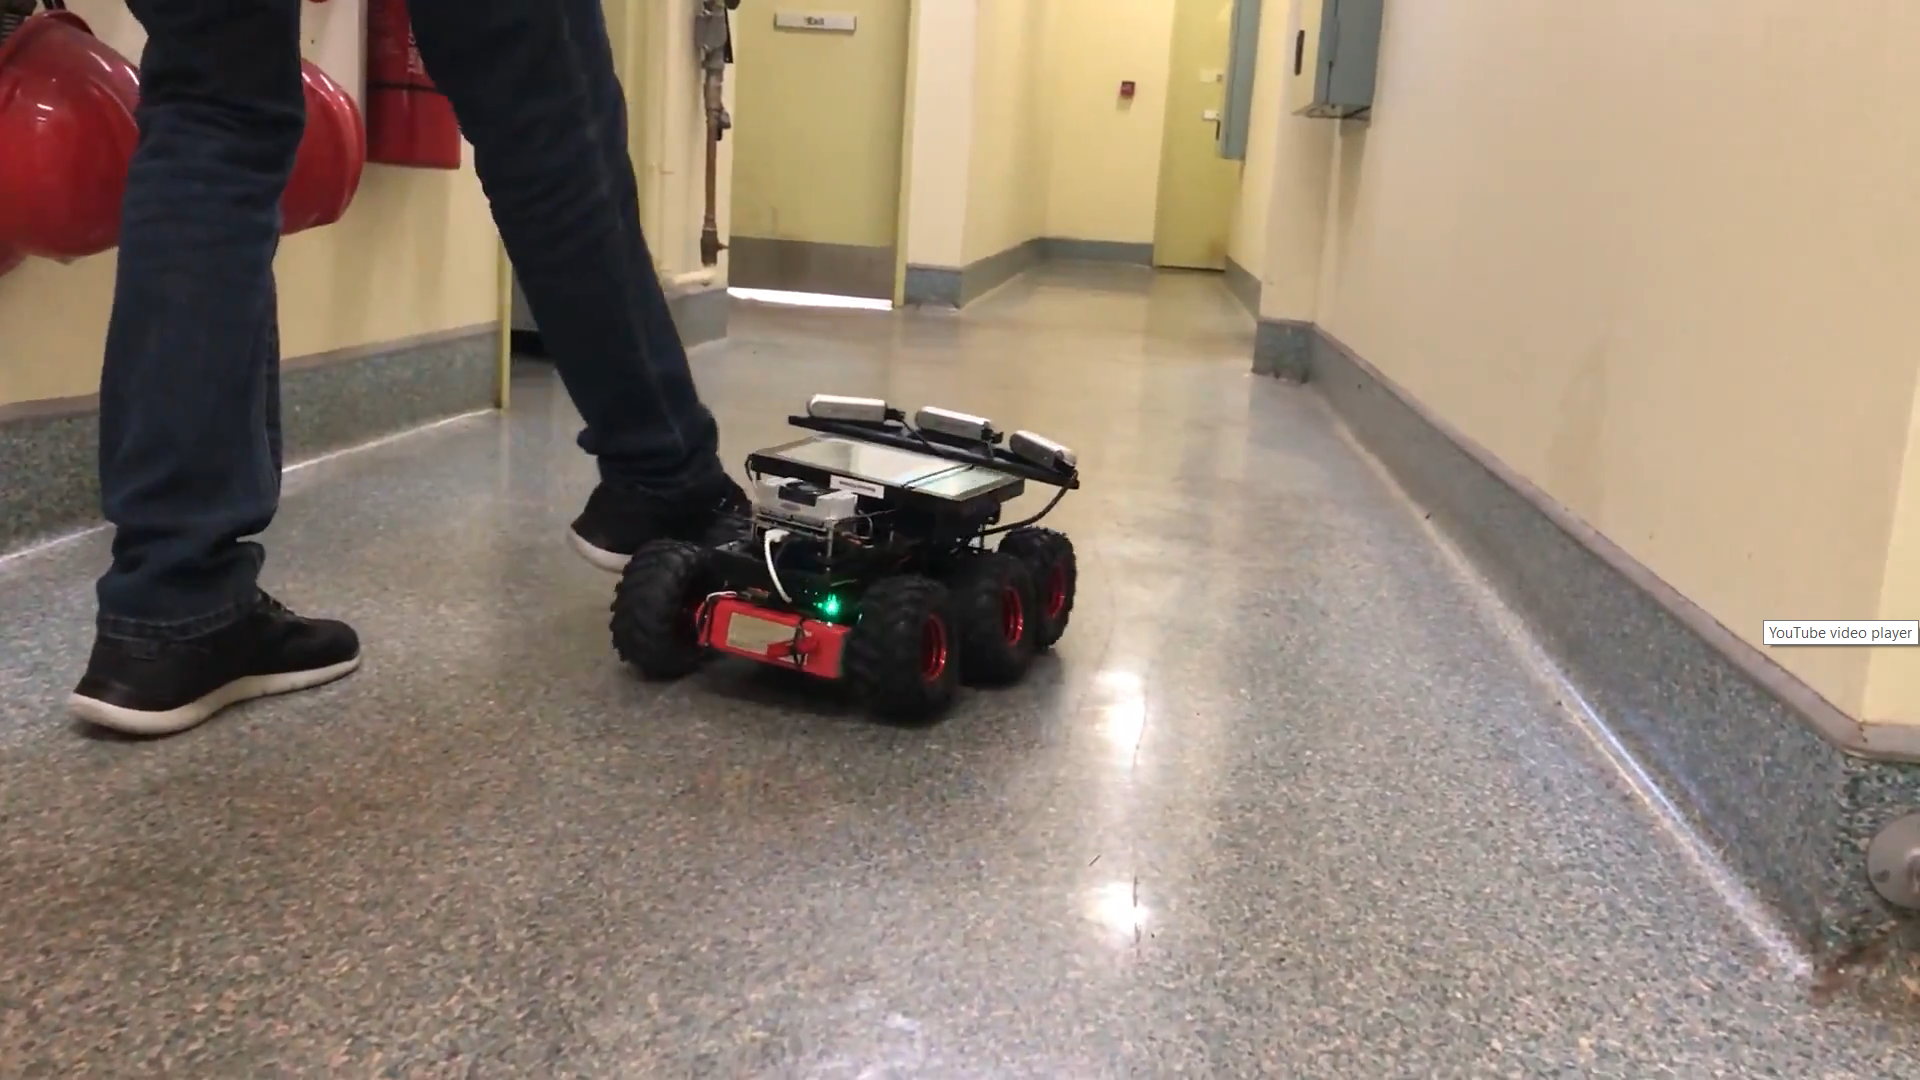
\includegraphics
        [width=.4\linewidth]
        {figures/wallie_self_run.png}
    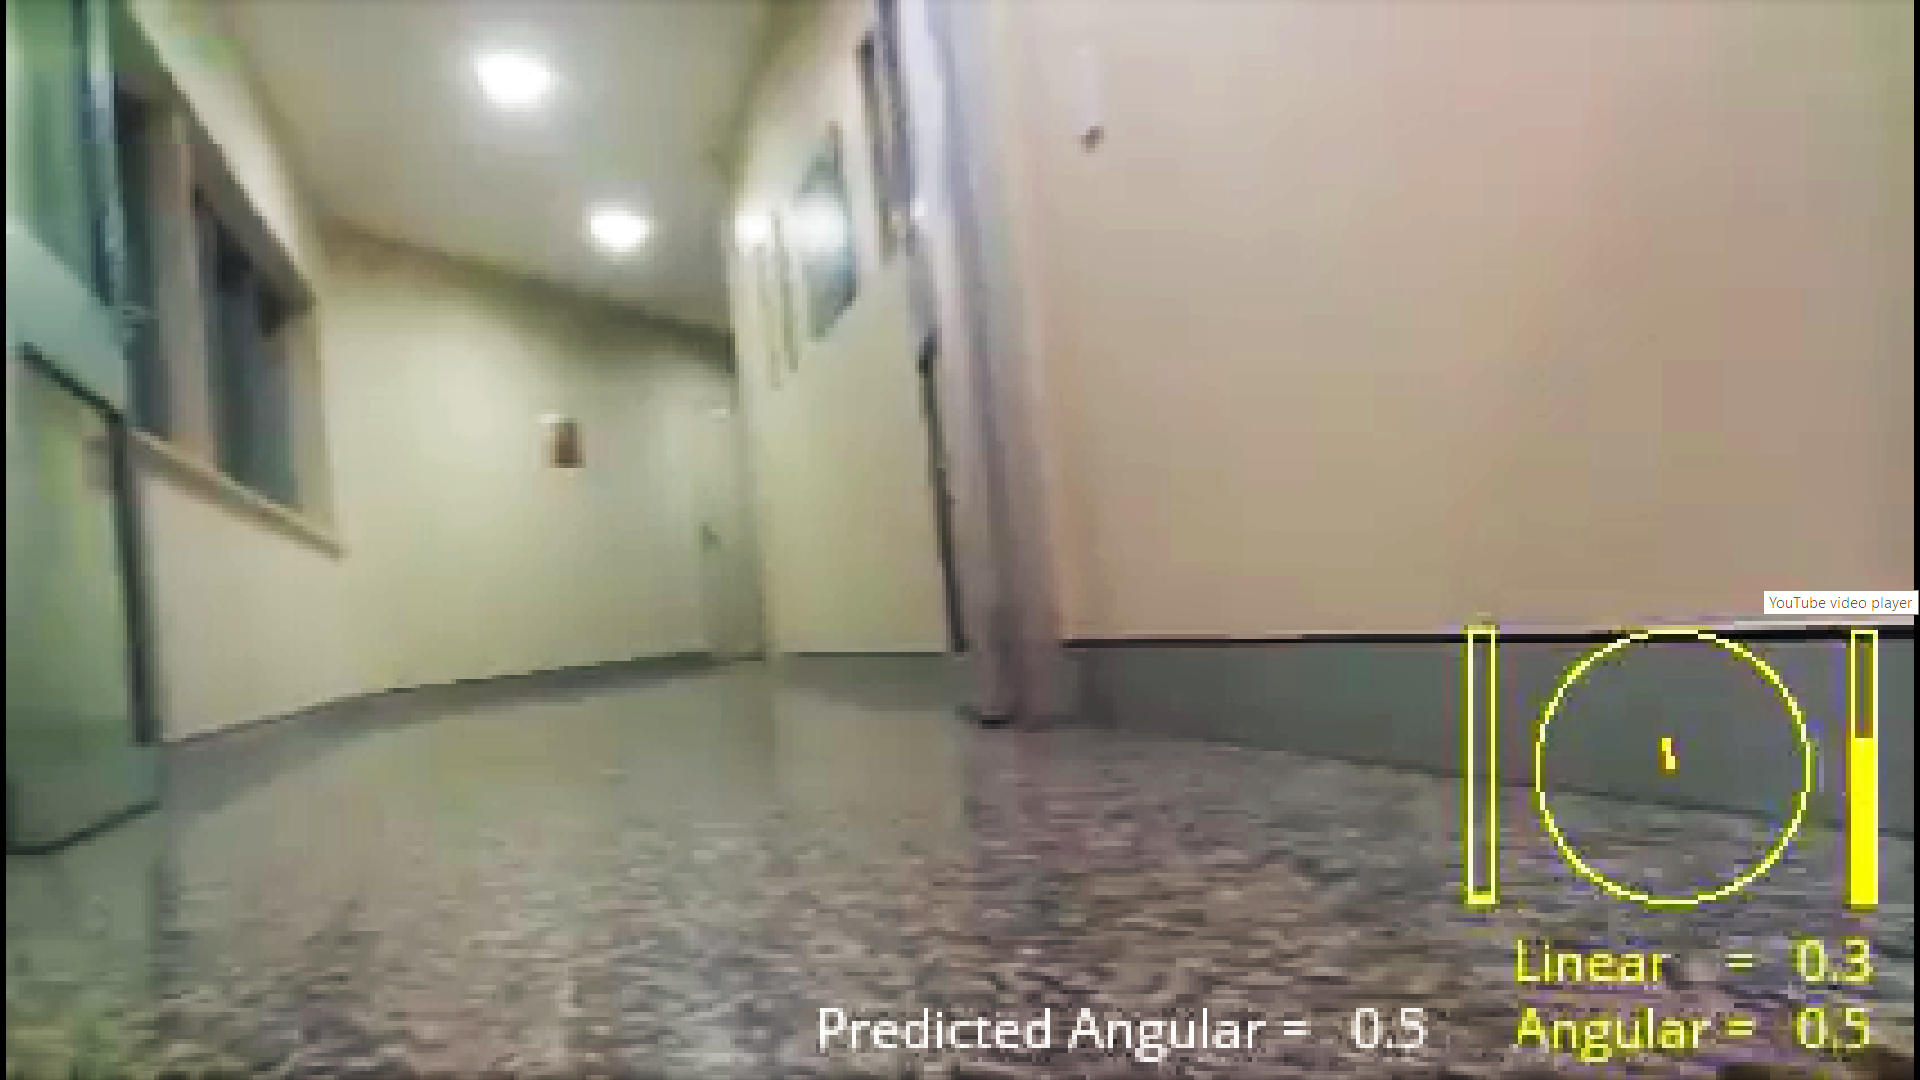
\includegraphics
        [width=.4\linewidth]
        {figures/trailnet_after_kick.png}
    \caption{Our indoor Trailnet CNN reacting to external disturbances}\vspace{-4mm}
    
\end{figure}

\paragraph{}
THe robot was tested in different hallways, including ones from where we did not collect training data. The robot performed remarkably well in cluttered hallways also, showing its robustness %to_cite% 
. In addition to that, the response to 90 degree corners was also remarkable, where the robot smoothly turned to follow the hallway.

% Image: Corners
\begin{figure}[H]
    \centering
    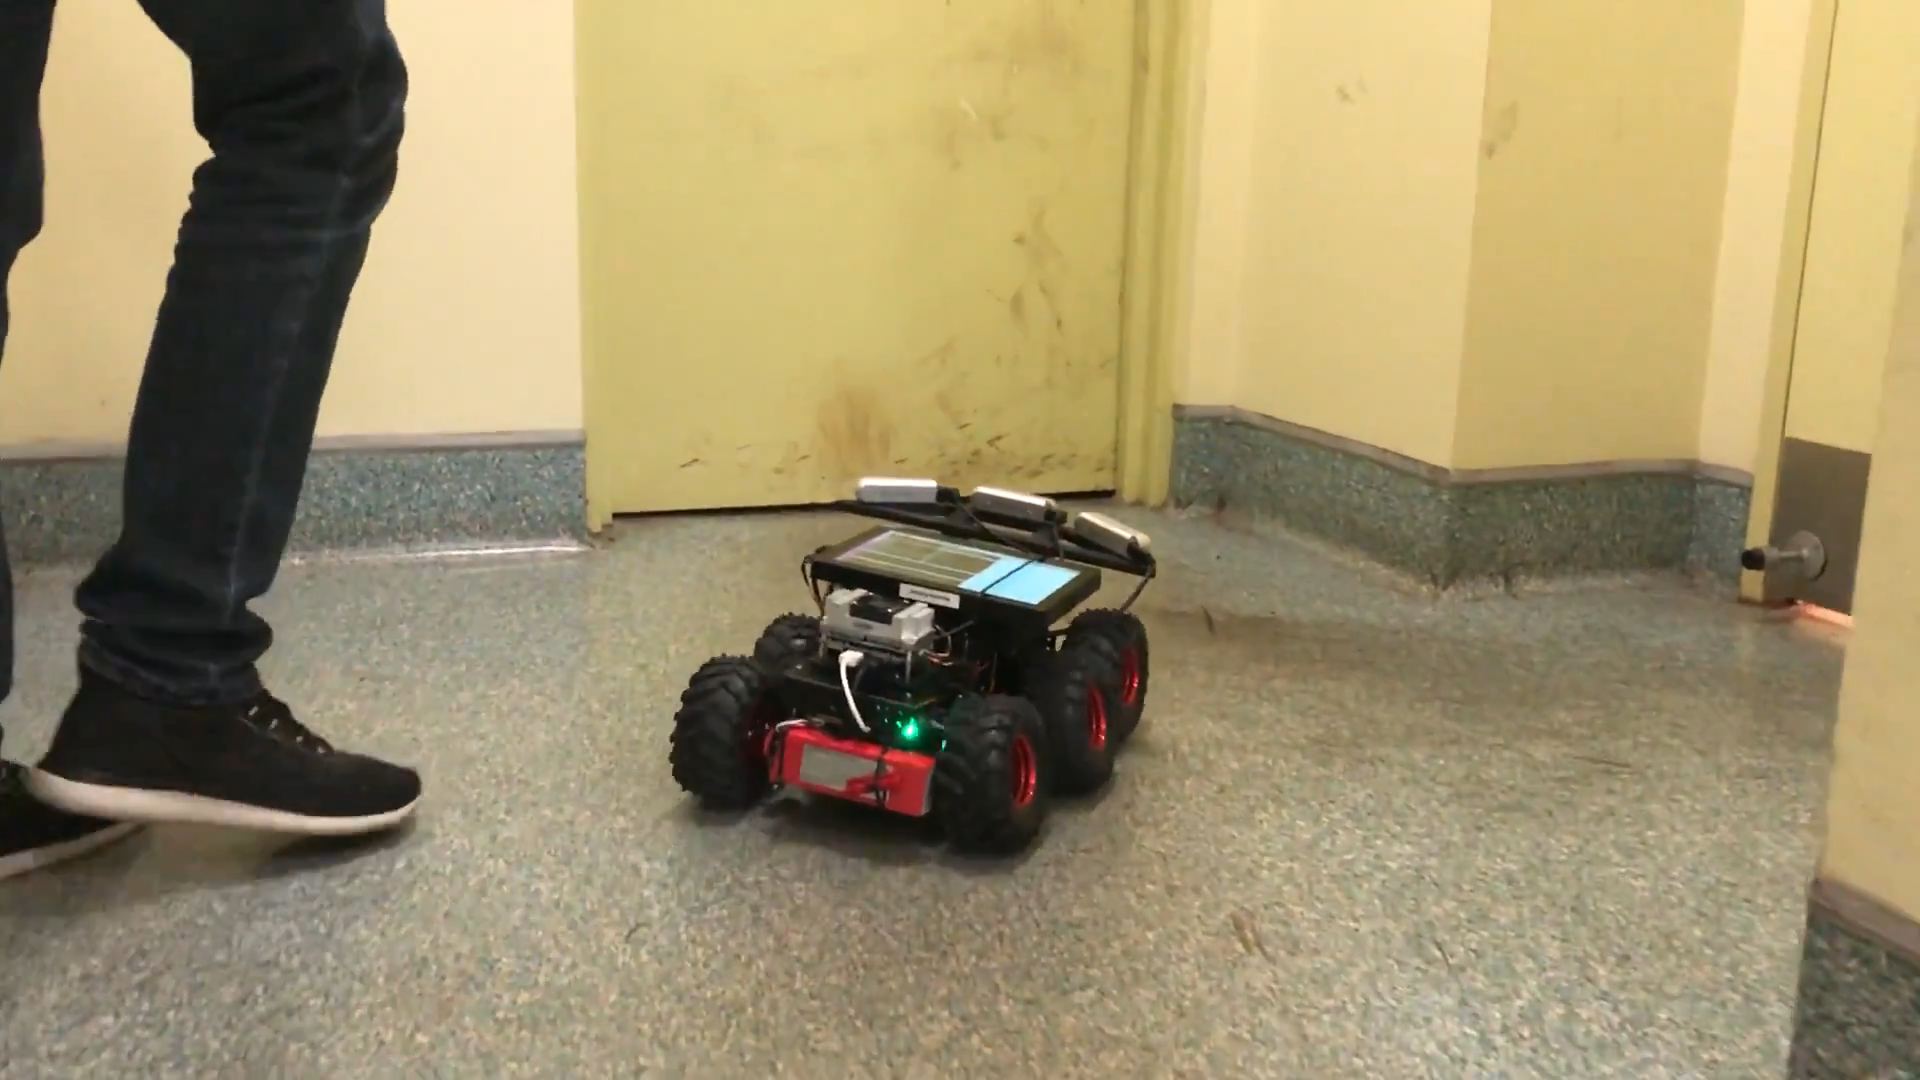
\includegraphics
        [width=6cm]
        {figures/wallie_self_turn.png}
    \caption{Our CNN reacting to corners}\vspace{-4mm}
    
\end{figure}

\paragraph{}
The results were presented to the fellow scientists in a Robotics Reading Group meeting as a demonstration of the end to end pipeline I designed. 
%!TEX root = ./intern_report.tex

\newpage
\subsection{Building Wallie: A Hardware Platform for Data Collection and Deployment}

\paragraph{}
The Robotics and Autonomous Systems Group of DATA61 is about field robotics. Therefore, it is not sufficient to demonstrate a concept theoretically or just by simulations. Instead, the members are expected to demonstrate our systems and results in complex real world environments.

\paragraph{}
Therefore, we needed a robot platform on which we can collect data and perform our tests. However, the available platforms of CSIRO were all in use for bigger projects. Hence we were requested to build a robot platform based on Pololu Wild Thumper chassis. This platform was previously assembled by our seniors: Isuru and Tharindu. However, as we describe below, we had to change almost every component of that to create a new robot to suit our specific needs. Our friend from Chile named this robot Wallie, in reference to the Wall-E movie and the fact our robot was initially built to follow walled hallways.

\begin{figure}[H]
    \centering
    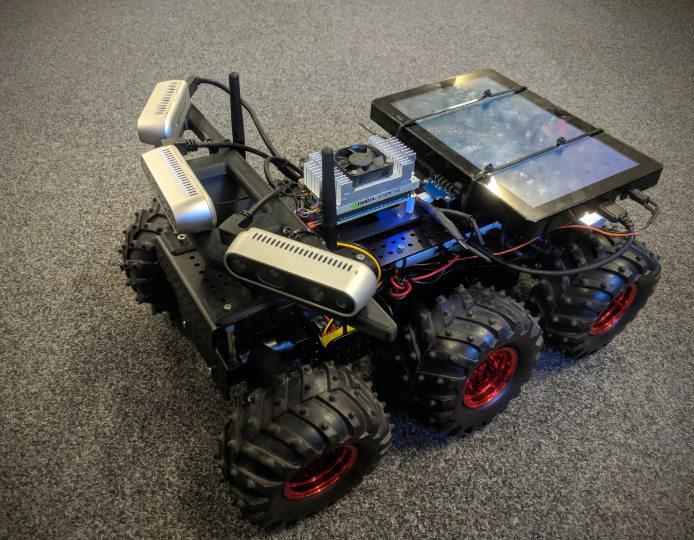
\includegraphics
        [width=10cm]
        {figures/wallie.PNG}
    \caption{Wallie: The Robot \label{Fig:wallie}}\vspace{-4mm}
\end{figure}

\paragraph{}
Firstly, we need a way to fix cameras in the robot for data collection and testing. I sketched a small camera rig to hold three Intel Realsense cameras, each facing: center, left and right at 30 degree angles from center. Samith Ashan, my coworker helped designed it in solidworks. That, a platform for the Jetson TX2 board and a holder for the Li-ion battery were then 3D printed. 

\subsubsection{Designing the Power Distribution System}

\begin{figure}[H]
    \centering
    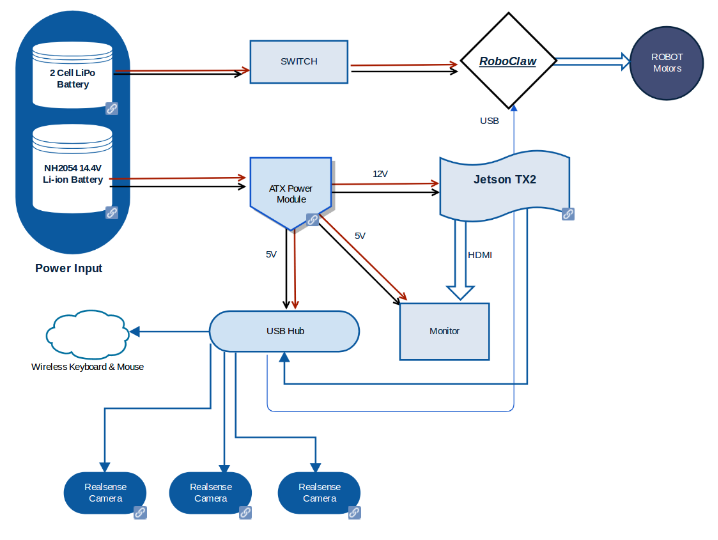
\includegraphics
        [width=13cm]
        {figures/wallie_hardware.PNG}
    \caption{Wallie: Hardware Hierarchy }\vspace{-4mm}
\end{figure}

\paragraph{}
We then designed a power distribution system for the robot, to deliver power from two batteries to all the sensors and actuators. We consulted Dr. Navinda and Mr. James Brett and came of with the following system. A 3 cell Li-Po delivers power to the Roboclaw Motor Controller, to which six 12V, 2.5D high torque motors are connected through a switch and a fuse (to prevent damage to the motor controller in case if the motors start stalling, as it happened once). The cameras and IMU are powered through an active USB hub. The USB hub LCD display and NVIDIA Jetson TX2 are powered through a robust power supply (12V, 5V) which is connected through a switch to the 7.4V Li-ion battery. Having two separate power sources for high-level and low-level systems helped through decoupling by reducing the chances of power failures from one network damaging the component in the other.

\paragraph{}
We documented the design of the robot in CSIRO's confluence wiki pages, so that fellow researchers can use it in the future for their own activities. Most of our time in CSIRO (about 75\%) was spent in building and debugging the robot platform. 


\subsubsection{NVIDIA Jetson TX2}

\paragraph{}
Jetson TX2 is device released by NVIDIA as a solution to run computation-intensive programs on board of a low power consuming device. This credit-card sized device contains CPU that can run AMD64 Linux, a powerful GPU that can run multiple neural networks at once using just 7.5W of power. DATA61 RAG is starting to unify and standardize their sensor and actuator APIs. Hence, they were considering NVIDIA's Jetson TX2 and Xavier as potential candidates for the high level controller on their multiple types of wheeled, legged and aerial robots.



% Table: Jetson
\begin{table}[H]
    \begin{center}
        \caption {NVIDIA Jetson TX2 Specifications} \label{tab:jetson}
        \begin{tabular}{|| r || l ||}    
            \hline
            GPU             & 256 CUDA cores of Pascal Architecture \\
            \hline
            CPU             & HMP Dual Denver 2/2 MB L2 + Quad ARM® A57/2 MB L2 \\
            \hline
            Memory          & 8 GB 128 bit LPDDR4, 59.7 GB/s \\
            \hline
            Data storage    & 32 GB \\
            \hline 
            USB             & USB 3.0 \\
            \hline 
            Connectivity    & Gigabit Ethernet, 802.11ac WLAN, Bluetooth \\
            \hline   
        \end{tabular}    
    \end{center}
\end{table}

\paragraph{}
Hence we began using Jetson TX2 as the high level controller with Orbitty carrier board. We flashed it with NVIDIA's Linux for Tegra kernel and set it up with Jetpack 3.2.1 (Updated to Jetpack 3.3 later).

% Image: Jetson
\begin{figure}[H]
    \centering
    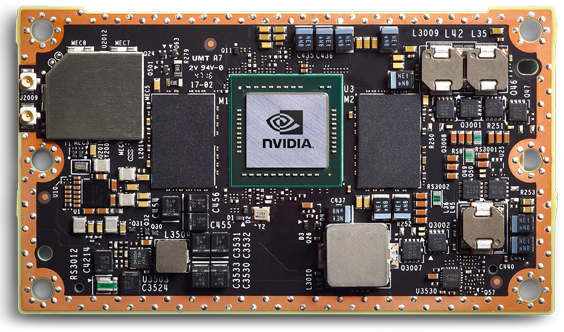
\includegraphics
        [width=8cm]
        {figures/jetson.png}
    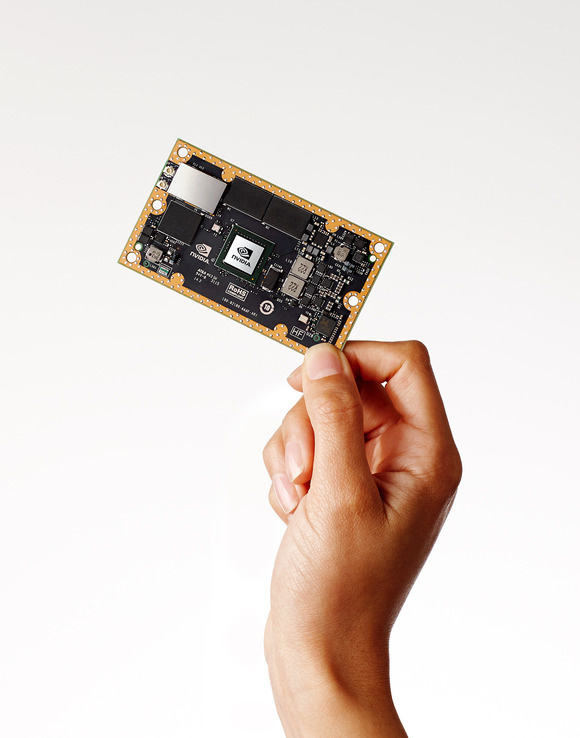
\includegraphics
        [height=5cm]
        {figures/jetson_scale.jpg}
    \caption{NVIDIA Jetson TX2 }\vspace{-4mm}
\end{figure}


\newpage
\subsubsection{Intel Realsense Depth Camera D435}

% Image: Realsense
\begin{figure}[H]
    \centering
    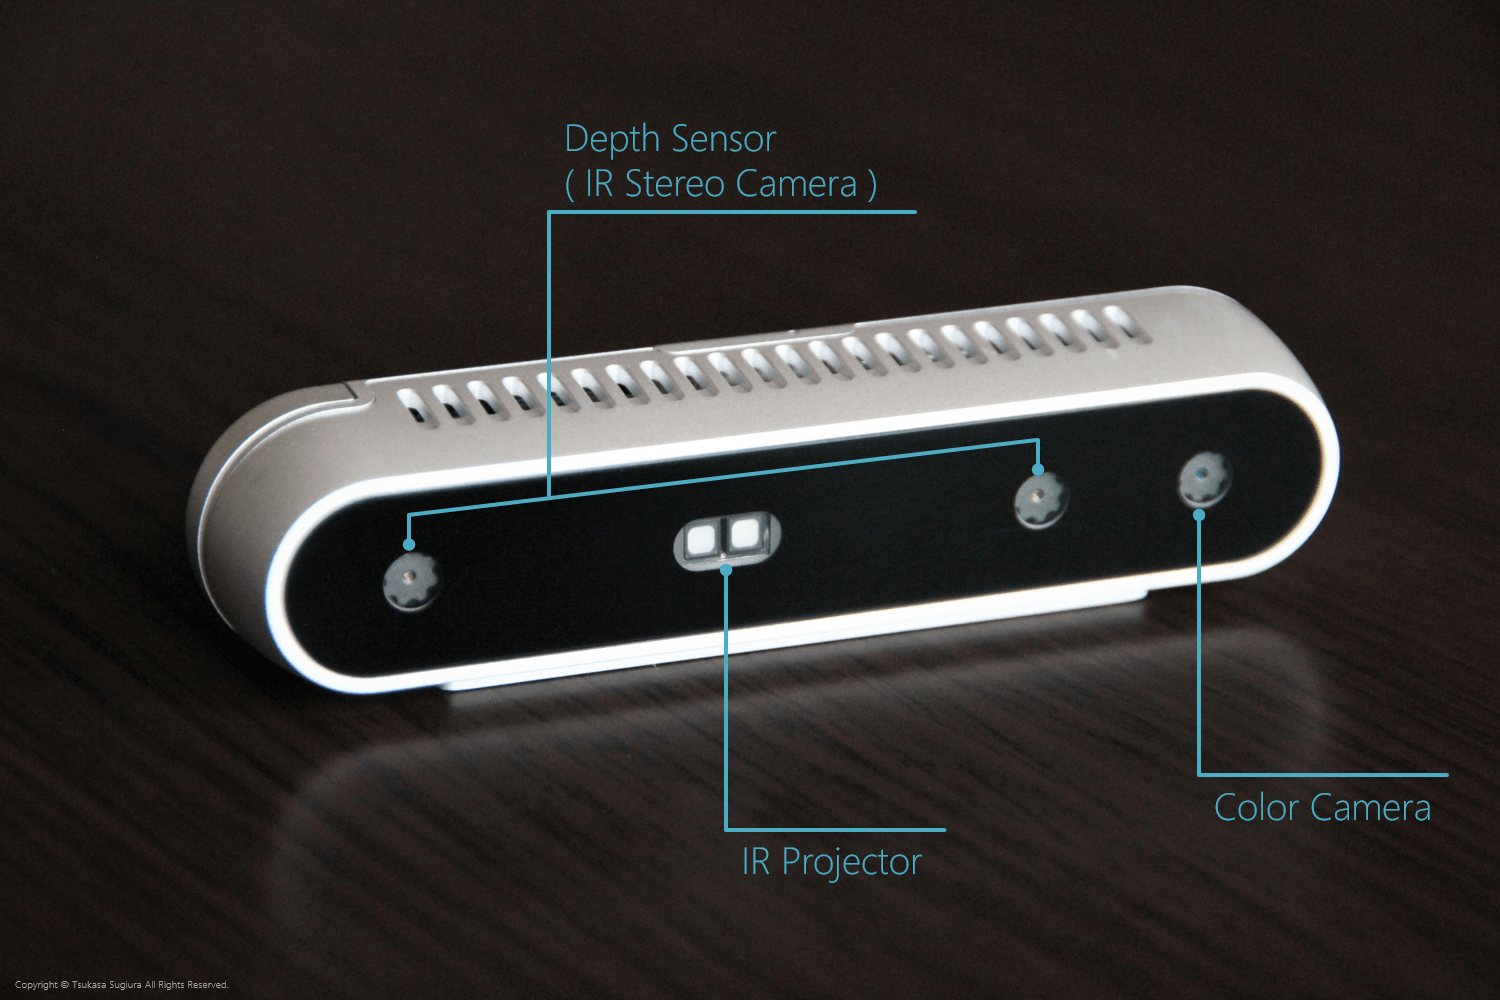
\includegraphics
        [width=8cm]
        {figures/realsense.png}
    \caption{Intel Realsense D435}\vspace{-4mm}
\end{figure}

\paragraph{}
Intel Realsense depth camera is able to output image streams of RGB, IR and Depth images as per following specifications. Due to the small size and versatility, RAG members considered using this as he de-facto vision sensor in low power robots. It can be connected to Jetson TX2 via a USB-C cable and there is an official ROS package from Intel with which it can communicate via serial and publish the image streams and diagnostic information.

% Table: Realsense
\begin{table}[H]
    \begin{center}
        \caption {Intel Realsense D435 Specifications} \label{tab:realsense}
        \begin{tabular}{|| r || l ||}
            \hline
            Depth FOV (Horz, Vert, Diag)	& 85.2\degree x 58\degree x 94\degree (+/- 3\degree) \\
            \hline
            Depth Stream Output Resolution	& Up to 1280 x 720 \\
            \hline
            Depth Stream Output Frame Rate	& Up to 90 fps \\
            \hline
            Maximum Range	                & Approx.10 meters \\
            \hline
            RGB   FOV (Horz, Vert, Diag)	& 69.4\degree x 42.5\degree x 77\degree (+/- 3\degree) \\
            \hline
            RGB   FOV (Horz, Vert, Diag)	& 1920 x 1080 at 30 fps \\
            \hline
            Connectors	                    & USB 3.0 Type - C \\
            \hline
        \end{tabular}    
    \end{center}
\end{table}

\paragraph{}
We used three of these cameras, each facing 30\degree left, right and center to collect image streams in ROSbags. We used RGB image stream to train our network, since most other robots do not have depth cameras as vision sensors. The depth data we collected was used by our coworker along with our IMU data for SLAM purposes.

\subsubsection{Roboclaw Motor Controller}

\paragraph{}
The wild thumper chassis we obtained had the arduino-based TREX motor controller on it. I spent few days trying to come up with an algorithm that can map the remote-control pulses to the PWM commands for smooth maneuvering. I succeeded partially. However, due to the problems described in the next section, we switched to Roboclaw controller, which mixes RC pulses into PWM using their proprietary algorithm.  

% Table: Roboclaw
\begin{table}[H]
    \begin{center}
        \caption {Pololu Roboclaw Motor Controller Specifications} \label{tab:roboclaw}
        \begin{tabular}{|| r || l ||}    
            \hline
            Motor channels              &   2   \\
            \hline
            Control interface           &	USB; TTL serial (2-way), RC pulses; PWM\\
            \hline
            Minimum operating voltage   &	6 V \\
            \hline
            Maximum operating voltage   &	34 V \\
            \hline
            Continuous output current per channel   &	30 A \\
            \hline
            Peak output current per channel         &	60 A \\
            \hline   
        \end{tabular}    
    \end{center}
\end{table}

\paragraph{}
The main advantage for choosing roboclaw was the availability of a compatible ROS package. However, we then found that the package was not being maintained for the past few years. I spent multiple weeks debugging the package and rewriting some of the driver code.

% Image: 2 motor controllers
\begin{figure}[H]
    \centering
    \begin{minipage}{.5\textwidth}
        \centering
        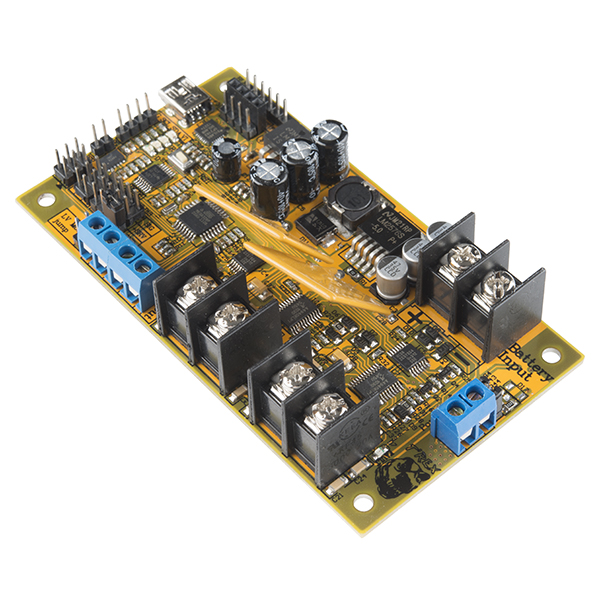
\includegraphics[width=0.8\linewidth]{figures/trex.jpg}
        \captionof{figure}{TREX Motor Controller}
        \label{fig:test1}
    \end{minipage}%
    \begin{minipage}{.5\textwidth}
        \centering
        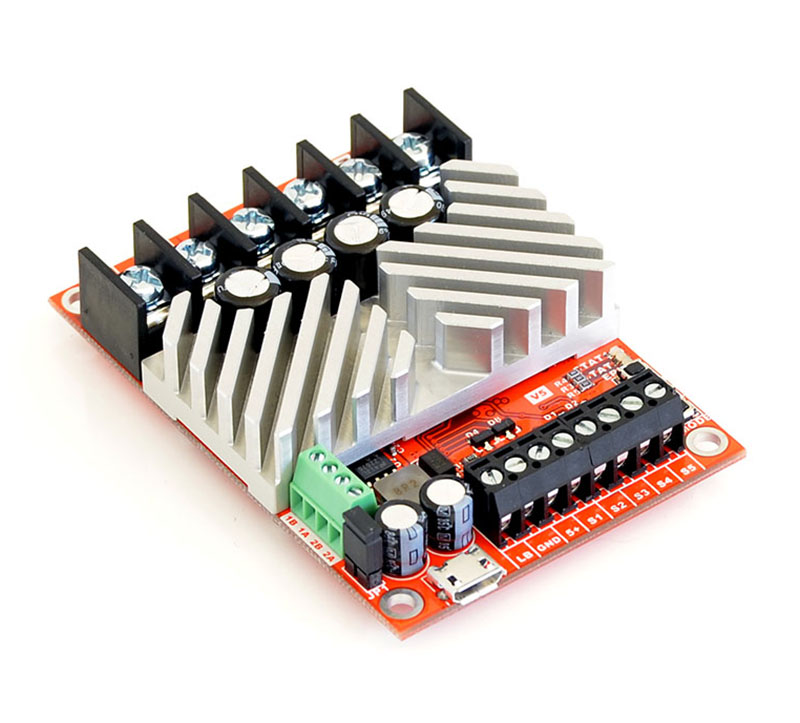
\includegraphics[width=0.8\linewidth]{figures/roboclaw.jpg}
        \captionof{figure}{Roboclaw Motor Controller}
        \label{fig:test1}
    \end{minipage}
\end{figure}

\subsubsection{Lord Microstrain IMU}


\newpage
\subsubsection{Problems Faced and Solutions}

\paragraph{}
Firstly, when we assembled wallie with TREX as the low level controller and a custom algorithm to mix RC signals into PWM values for motor control, we found that it was quite difficult to maneuver the robot. Using remote control, we could not make it take tight turns at corners and the robot did not turn smoothly in carpeted floors due to friction. We found three problems that resulted in this:

\begin{itemize}
    \item Center of mass of the assembled robot was not exactly at the geometric center.
    \item RC mixing algorithm is not robust enough
    \item The MOSFET switch used between the battery and TREX limits the current, reducing the torque of motors.
\end{itemize} 

\paragraph{}
To solve these issues, I improved the mixing algorithm, Uvindu reassembled the robot and we removed the switch. The performance improved, but after few hours of test run, the TREX controller burnt off. Dr. Navinda instructed us to troubleshoot it and submit a report. After intensive testing and discussion with James Brett, Pubudu Aravinda and Samith Ashan, we identified the key issue as the in-built fuses of the old TREX board that failed to function as a large current was drawn when motors stalled on the rough carpet floor. As a result, the hall sensor on the controller got burnt, short circuiting and damaging two MOSFETs on the same side of the H-bridge. Dr. Navinda accepted the report and ordered the Roboclaw controller as replacement (since TREX boards are outdated and unavailable in the market). 

\paragraph{}
The prime advantage of the new Roboclaw was the associated ROS package. However, we soon found that the public package was severely outdated and not maintained. I contacted the manufacturers of Roboclaw and got a copy of the ROS package they use internally. That package also had several issues which we struggled with, throughout the project. After a week of debugging, I realized a main issue was that their driver was not thread safe. That is, when the ROS node receives a message, it runs the specified callback function, which is initiated on a new thread. If multiple such function calls are made in quick succession, it results in multiple threads that try to access the same resources (serial port). This results in unexpected frequent crashes. I changed the driver package to be thread safe and fixed some issues with incompatibility between velocity commands and odometry readings.

\paragraph{}
The D435 Realsense cameras are also not error free. We noticed that their output serial stream hangs unexpectedly and the only known solution is to unplug and plug them back. After some reading, I found that this is a hardware bug addressed by Intel as unfixable on this device. Therefore, I recommended Nick to not rely on these devices for critical tasks, such as the DARPA subterranean challenge.

\paragraph{}
When collecting data for hill climbing, I noticed a large variance (noise) in the IMU readings. Since our neural networks consider only the current inputs to provide instantaneous output velocity, noise in such an input would hinder the training process as the optimizer struggles to find correlation. I noticed that this high variance was due to the small slope of the hills and the increase in the percentage error due to that. To avoid this, I suggested fixing the IMU at an elevated angle to the horizontal on the robot.

\paragraph{}
We also faced issues with Jetson TX2, since the orbitty development board which we had to use (due to its small form factor) had its own modified Linux kernel. Many drivers were not directly supported for this and we had to modify the kernel to install certain drivers.
%!TEX root = ./intern_report.tex

\newpage
\subsection{Designing and Implementing an Efficient End-toEnd Pipeline for Machine Learning in Robotics}

\begin{figure}[H]
    \centering
    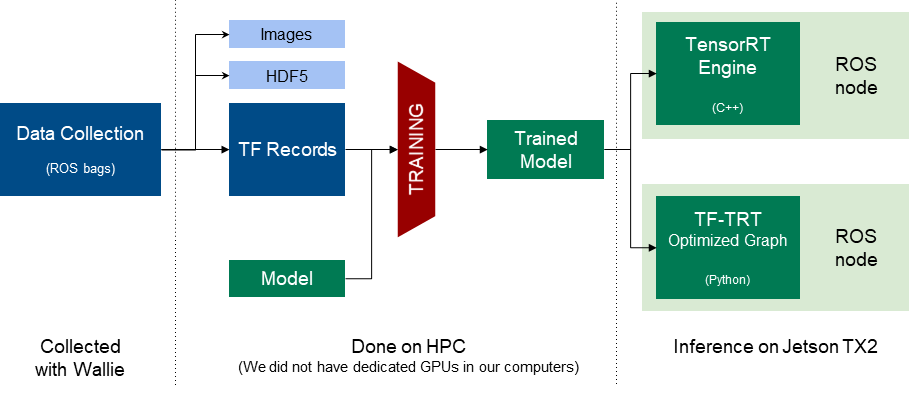
\includegraphics
        [width=16cm]
        {figures/full_pipeline.PNG}
    \caption{End-to-End Pipeline \label{Fig:pipeline}}\vspace{-4mm}
\end{figure}

\subsubsection{Training on Supercomputers}
\label{training_on_Supercomputers}

\subsubsection{TF Records}

\begin{figure}[H]
    \centering
    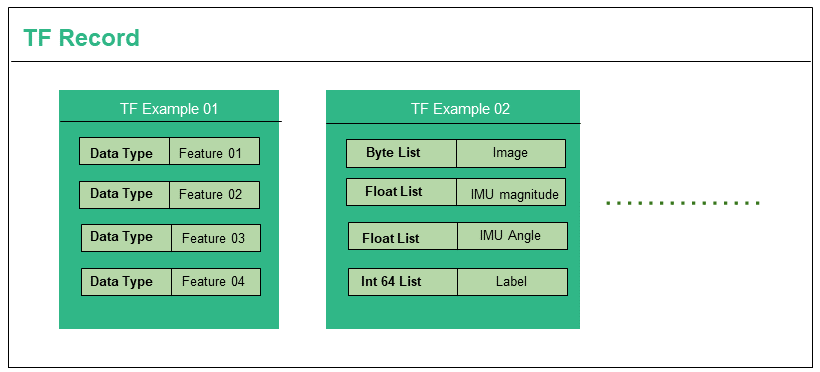
\includegraphics
        [width=9cm]
        {figures/tfrecord_structure.PNG}
    \caption{Structure of a TF Record}\vspace{-4mm}
\end{figure}

\begin{figure}[H]
    \centering
    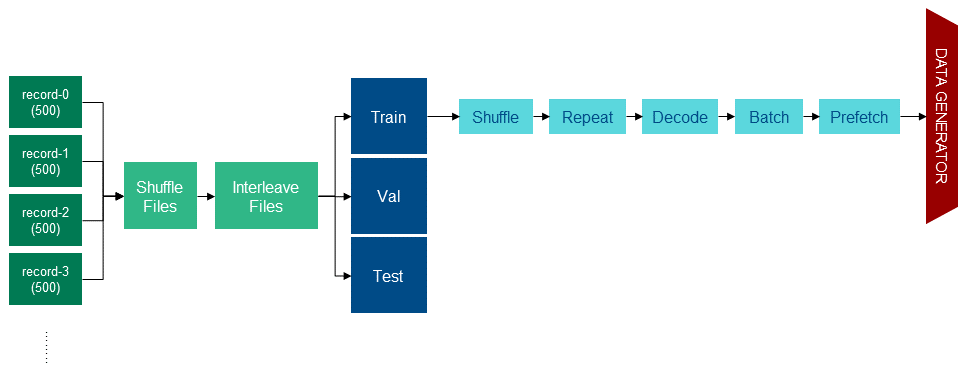
\includegraphics
        [width=16cm]
        {figures/input_pipeline.PNG}
    \caption{Data Input Pipeline with TFRecords}\vspace{-4mm}
\end{figure}


\subsubsection{TensorRT: Deployment on a low power device}
\label{tensorrt}

\begin{figure}[H]
    \centering
    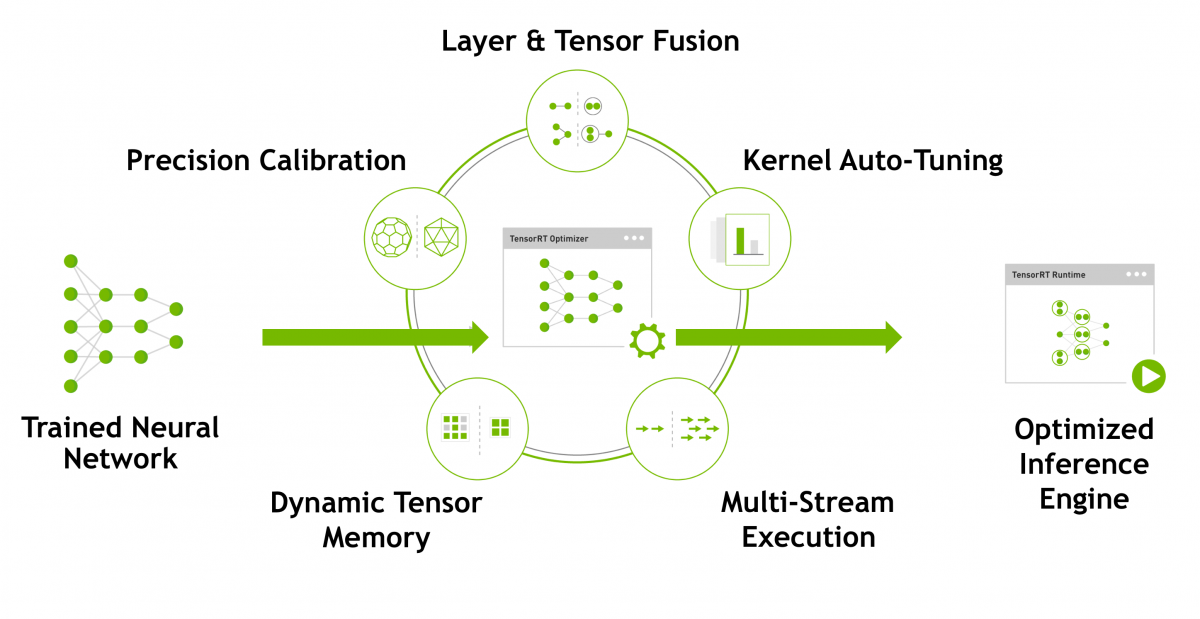
\includegraphics
        [width=13cm]
        {figures/trt.png}
    \caption{TensorRT in a nutshell}\vspace{-4mm}
\end{figure}

\begin{figure}[H]
    \centering
    
\includegraphics
        [width=13cm]
        {figures/deploy_pipeline_cpp.PNG}
    \caption{Deployment Pipeline: C++}\vspace{-4mm}
\end{figure}

\begin{figure}[H]
    \centering
    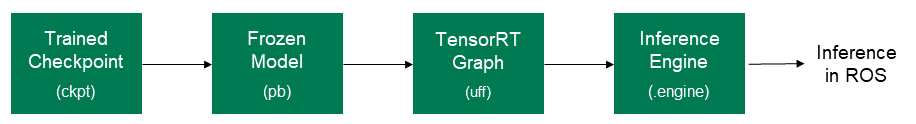
\includegraphics
        [width=13cm]
        {figures/deploy_pipeline_python.PNG}
    \caption{Deployment Pipeline: Python}\vspace{-4mm}
\end{figure}

\subsubsection{Problems Faced and Solutions}
%!TEX root = ./intern_report.tex

\newpage
\subsection{Hillnet: An Experimental Attempt at Utilizing ML for Hill Climbing}

\paragraph{}
After successfully demonstrating indoor-Trailnet built from scratch, trained and deployed with my pipeline, our supervisor Nick described about his idea of experimenting with a algorithm to climb hills while avoiding obstacles using computer vision. We were asked to come up with a system where two different types of inputs are merged: scaler inputs representing the direction of the slope and the RGB image input from a camera to output a velocity command to control the motor controller. Trailnet, which itself was based on resnet-18 was chosen to be modified to build such a neural network.

\subsubsection{Preprocessing IMU and Velocity Data}

\paragraph{}
The LORD Microstrain IMU sends its data through serial to its ROS package, which publishes the IMU readings in two types: as a quaternion and set of cartesian x,y,z vector components of perceived acceleration. I decided to use the vector components to calculate the magnitude and direction of the gravity vector projected on the horizontal plane of the robot. Direction $\theta \in [-\pi, \pi]$ was measured with respect to the heading direction and then converted to $[0, 1]$ range using the sigmoid function to match the range of the other normalized inputs. I chose to output the angular velocity as a float $\in [0,1]$ using a sigmoid output node (in classification approach) and scale it to the necessary angular Velocity.

\begin{align*}
    x, y, z   &= \text{Magnitude of the cartesian components of perceived acceleration. x: forward, z: vertical} \\
    r, \theta &= \text{polar components of the acceleration vector projected on the horizontal plane of robot} \\
    r_{in}, theta_{in}     &= \text{processed values given as input to the network}
\end{align*}

\begin{align*}
    r &= \sqrt{x^2 + y^2} \\
    r_{in} &= \tfrac{r}{g} & \text{normalized by the maximum: g} \\
    \theta &= \arctan({\tfrac{y}{x}})     &  \theta \in [-\pi,\pi] \\
    \theta_{in} &= \text{sigmoid}(\theta) &  \theta_{in} \in [0,1]
\end{align*}


\newpage
\subsubsection{Data Collection}

\paragraph{}
As per the instructions of our supervisor, Uvindu collected data in the slopes around CSIRO campus during the last few weeks of the internship. He placed the robot on the bottom of the hill and drove the robot following the steepest ascent. When he faced an obstacle, he went around the obstacle and continued to follow the steepest ascent. Image streams from the camera, IMU data and the odometry reading from the motor encoders were recorded in ROSbags.

% Image: Data Collect
\begin{figure}[H]
    \centering
    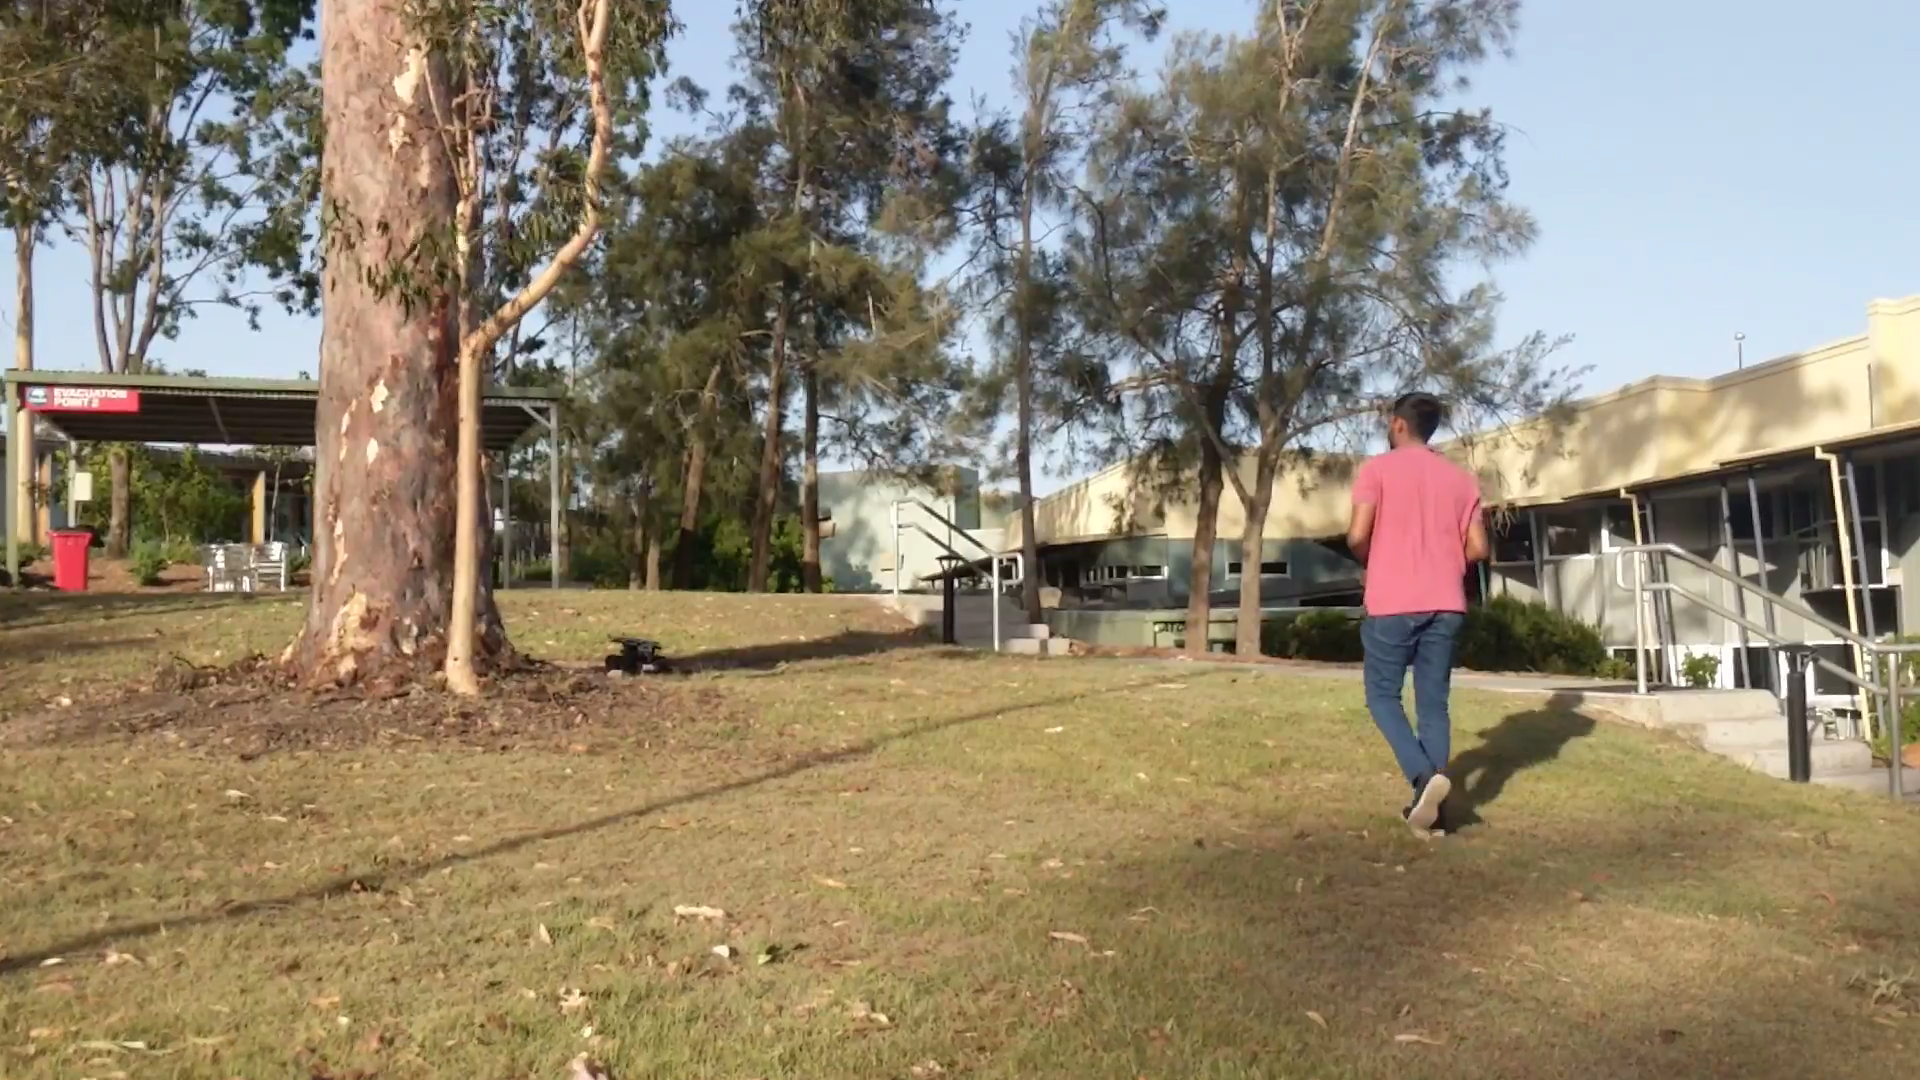
\includegraphics
        [width=8cm]
        {figures/hillnet_data_collect.png}
    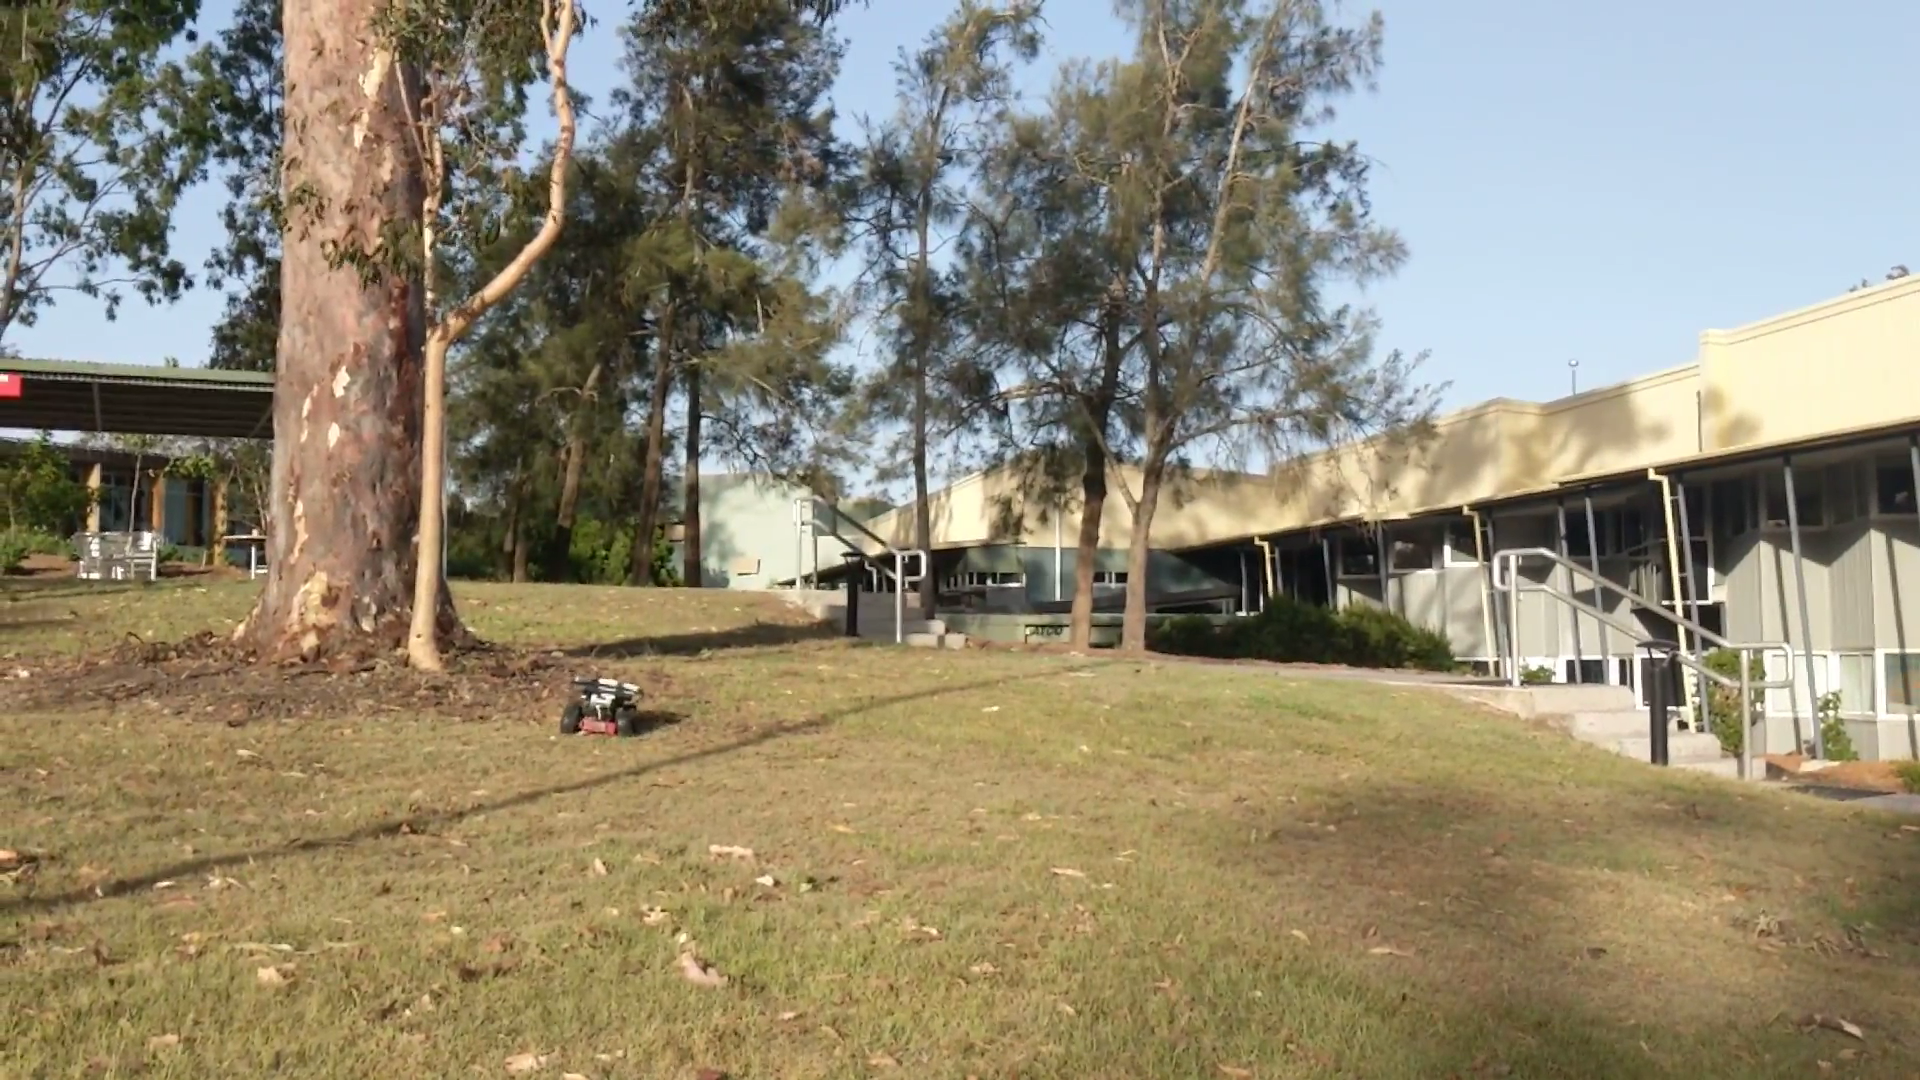
\includegraphics
        [width=8cm]
        {figures/hillnet_data_collect_2.png}
    \caption{Data Collection to Train Hillnet}\vspace{-4mm}
\end{figure}

\subsubsection{Merging Scaler and Image Inputs}

\paragraph{}
For this task, it was necessary to decide how the two types of inputs: scaler and image are combined in the neural network. Our supervisor proposed a method, where the IMU values are concatenated to the flattened output of the convolution layers, followed by few fully connected layers. The inspiration for this idea comes from the insight that deeper layers of a deep neural network identify higher level features and therefore the flattened average pooling output of the CNN should be containing information about by how much should the robot turn to avoid the obstacle. Therefore, concatenating the IMU inputs, which also tell by how much the robot should turn to follow the hill and following it with few fully connected layers might result in the network learning an OR operation between two inputs. 

\paragraph{}
However, a research paper on merging these kind of inputs ~\cite{hand_eye} proposed an alternative method, where the scaler inputs are broadcasted into a matrix with the right size, processed by few fully connected layers and added elementwise to the output of an intermediate layer in the CNN. The insight behind this is the fact that the output of the fully connected layers might act like a mask on the image, effectively clouding and directing the decision process of the CNN. After some consideration and experimentation, we decided to follow our supervisor's method since it was more suitable for our task.


% Image: Merge Inputs
\begin{figure}[H]
    \centering
    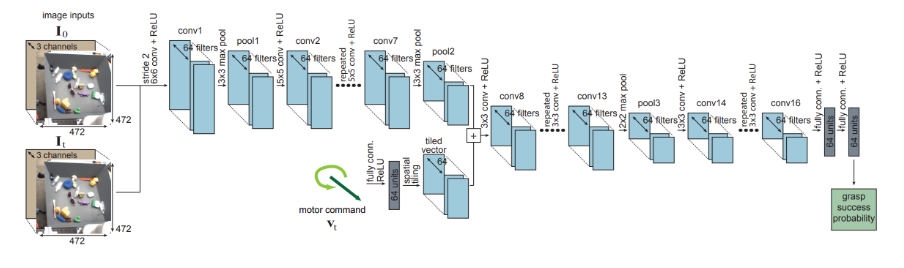
\includegraphics
        [width=16cm]
        {figures/merge_inputs.PNG}
    \caption{Merging by Broadcast and Add Elementwise as a Mask}\vspace{-4mm}
    
\end{figure}

\subsubsection{Regression Approach}

\paragraph{}
Next we brainstormed on how to post-process the output of the network to steer the robot. During the discussion, our supervisor first suggested to use the regression approach. That is, to build a network with a single output node that has no activation function, so the output value can be directly used as the angular velocity command to steer the robot. This is quite straightforward to build, train and test. The neural network can be trained with IMU and Image data and output as the angular velocity from odometry reading when driven by remote control during data collection.

% Image: Regress Architecture
\begin{figure}[H]
    \centering
    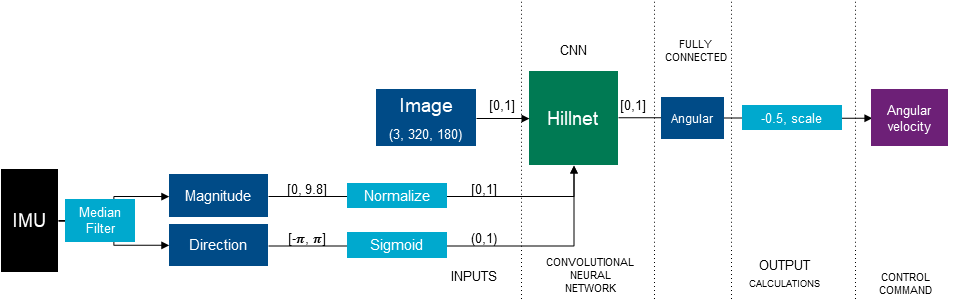
\includegraphics
        [width=16cm]
        {figures/hillnet_regress.PNG}
    \caption{Hillnet Regression Architecture}\vspace{-4mm}
    
\end{figure}

\subsubsection{Classification Approach}

\paragraph{}
During that discussion, I suggested trying a classification approach similar to that of trailnet. First advantage was the ability to fine tune the output by adjusting the constants. With regression, either it works or not. But with classification, we could fine tune it to work as we wish. Then, the effect of human error introduced in collecting data can be made insignificant by quantizing the angular velocity into classes: left, center and right. 

% Image: Classify Architecture
\begin{figure}[H]
    \centering
    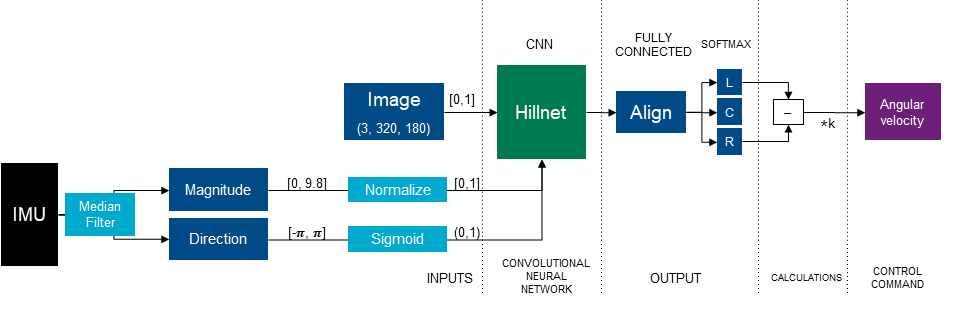
\includegraphics
        [width=16cm]
        {figures/hillnet_classify.PNG}
    \caption{Hillnet Classification Architecture}\vspace{-4mm}
    
\end{figure}

\paragraph{}
Next, I proposed a scheme of augmenting data to effectively triple the amount of collected training data. That is, first we record image streams from all three cameras. Then, in the input pipeline, I made changes to add +30\degree and -30\degree to the IMU angle and use it as datapoints along with the image streams from left and right cameras respectively. This would train the network to NOT turn away from the steepest slope, unless an obstacle is encountered, I argued. Our supervisor accepted the idea and asked me to work on both classification and regression in parallel to compare their merits. 



\subsubsection{Problems Faced and Solutions}

\paragraph{}
First problem we faced was the human errors in data collection. Since the hills had a small slope, Uvindu had difficulty in visually identifying the highest-slope direction and steering the robot towards it. When we analysed the collected data using the visualization techniques, we found there was a steady state error by up to 5\degree-10\degree. We tried collecting more data with a couple of days remaining to end the internship.

\paragraph{}
Another anomaly I observed from the visualization was the fact the IMU input had a high variance (noise). This was due to facts the slope was gentle (high percentage error) and the spring loaded suspension system of Wallie was causing it to wobble, introducing low frequency vibrations. This was critical, since our neural network does not remember nor correlate with the past inputs, but considers only the current inputs to give instantaneous outputs. Such a noisy input will prevent the training process from converging to a global maxima. Hence I suggested mounting the IMU at an angle to reduce the percentage error. After experimenting with mean and median filters of various lengths, I implemented a median filter of length 50 to smoothen the noise.

\paragraph{}
On the last few days of the internship, while debugging the network, I accidentally noticed that our collected dataset had an unhealthy disparity. That is, only 0.15\% data accounted for avoiding obstacles, while the rest 99.85\% accounted for climbing following the steepest hill. This is a classic problem in data science where the neural network simply learns to suggest "go forward" and be right 99.85\% of the time! I had discussed a similar potential problem with the supervisor at the beginning of the project, where I raised concerns that "we are not showing the robot which input-output combinations are wrong. we are showing only what is right". Our supervisor assured that "the robot will learn what is wrong, when you turn the robot to face the hill after avoiding an obstacle". However, the percentage of that kind of data was dwarfed by the "straight climbing" data in the dataset. I discussed this with Micheal and our supervisor and started implementing my idea of artificially boosting the frequency of "avoiding obstacle" data in the input pipeline.

\paragraph{}
However, we were running out of time by the end of the internship to try all possible ideas and experiment with all the possibilities. I stayed for multiple days overnight at office to try and finish as much as possible, but we couldn't try everything within that short time. Spending most of our time on building and debugging the robot platform could be one of the reasons for our time being limited for exploring new ideas with Hillnet. However, we realized that this is quite common in experimental field robotics, where scientists get to spend most of the time struggling with the hardware issues. 
%!TEX root = ./intern_report.tex

\newpage
\subsection{Life at CSIRO}

\paragraph{}
CSIRO, being a world class research institute, thrives to create a stress-free work environment that encourages people to socialize and to boost creativity. There is a workplace culture in DATA61 to bring cakes (or any equivalent sweets) for all the coworkers if one gets married, arrive at CSIRO, leave CSIRO, has a birthday and so on. I shared Sri Lankan sweets (sent by my mother in mail) for my birthday and cakes with everyone for arriving at and leaving CSIRO.

\subsubsection{Reading Groups and DATA61 Meetings}

\paragraph{}
Every friday, a small meeting called "Robotics Reading Group" is hosted, where one scientist explains his current project to everyone who attends the meeting. This way, we get to know the latest technology that is being developed in different parts of DATA61 and new projects that are being started. This meeting also allows the scientist to be questioned, so that he can derive insights from the audience and refine his procedures in the future. Also, once in a fortnight our supervisor Nick holds a "ML Robotics" meeting for all engineers working on machine learning. There we discuss our current ideas and issues to help each other. In addition to these, there are monthly meetings with the entire CSIRO (branches from all over Australia join via video conferencing), where new developments are discussed. One such meeting had the lead scientist from NASA's Insight Mars Lander mission as the chief guest explaining the challenges faced in their mission and taking our questions on the matter.

\begin{figure}[H]
    \centering
    
\includegraphics
        [width=12cm]
        {figures/presentation.png}
    \caption{Presenting the Pipeline in Robotics Reading Group}\vspace{-4mm}
\end{figure}

\subsubsection{Presenting the Pipeline at Reading Group to the Scientists}

Uvindu and I presented the pipeline to other scientists during one of the last Reading Group meetings of the year. It was well received, thanks to the support of our supervisor who encouraged others to use our pipeline in their workflow. Many asked questions and were convinced of the merits of such a unified framework. I had a few scientists reaching out to me on the following days asking me to develop visualization tools to complement the pipeline. 

\subsubsection{DATA61 Live Event}

DATA61 Live is an event held annually to showcase the science and technology innovations of DATA61 from all over Australia. In 2018, it was held in Brisbane, in our city. The theme was: 'Adapting to Disruption'. We signed up as volunteers and apart from volunteering, we had a chance to attend many lectures, talks and forums. It was a great experience.

\begin{figure}[H]
    \centering
    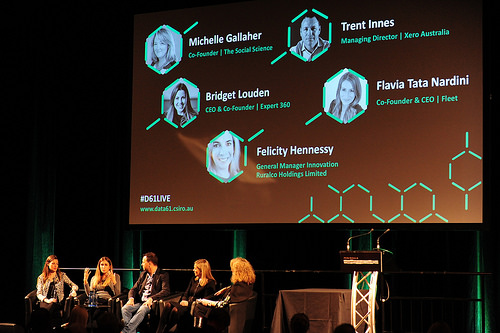
\includegraphics
        [height=5cm]
        {figures/data61_live_1.jpg}
    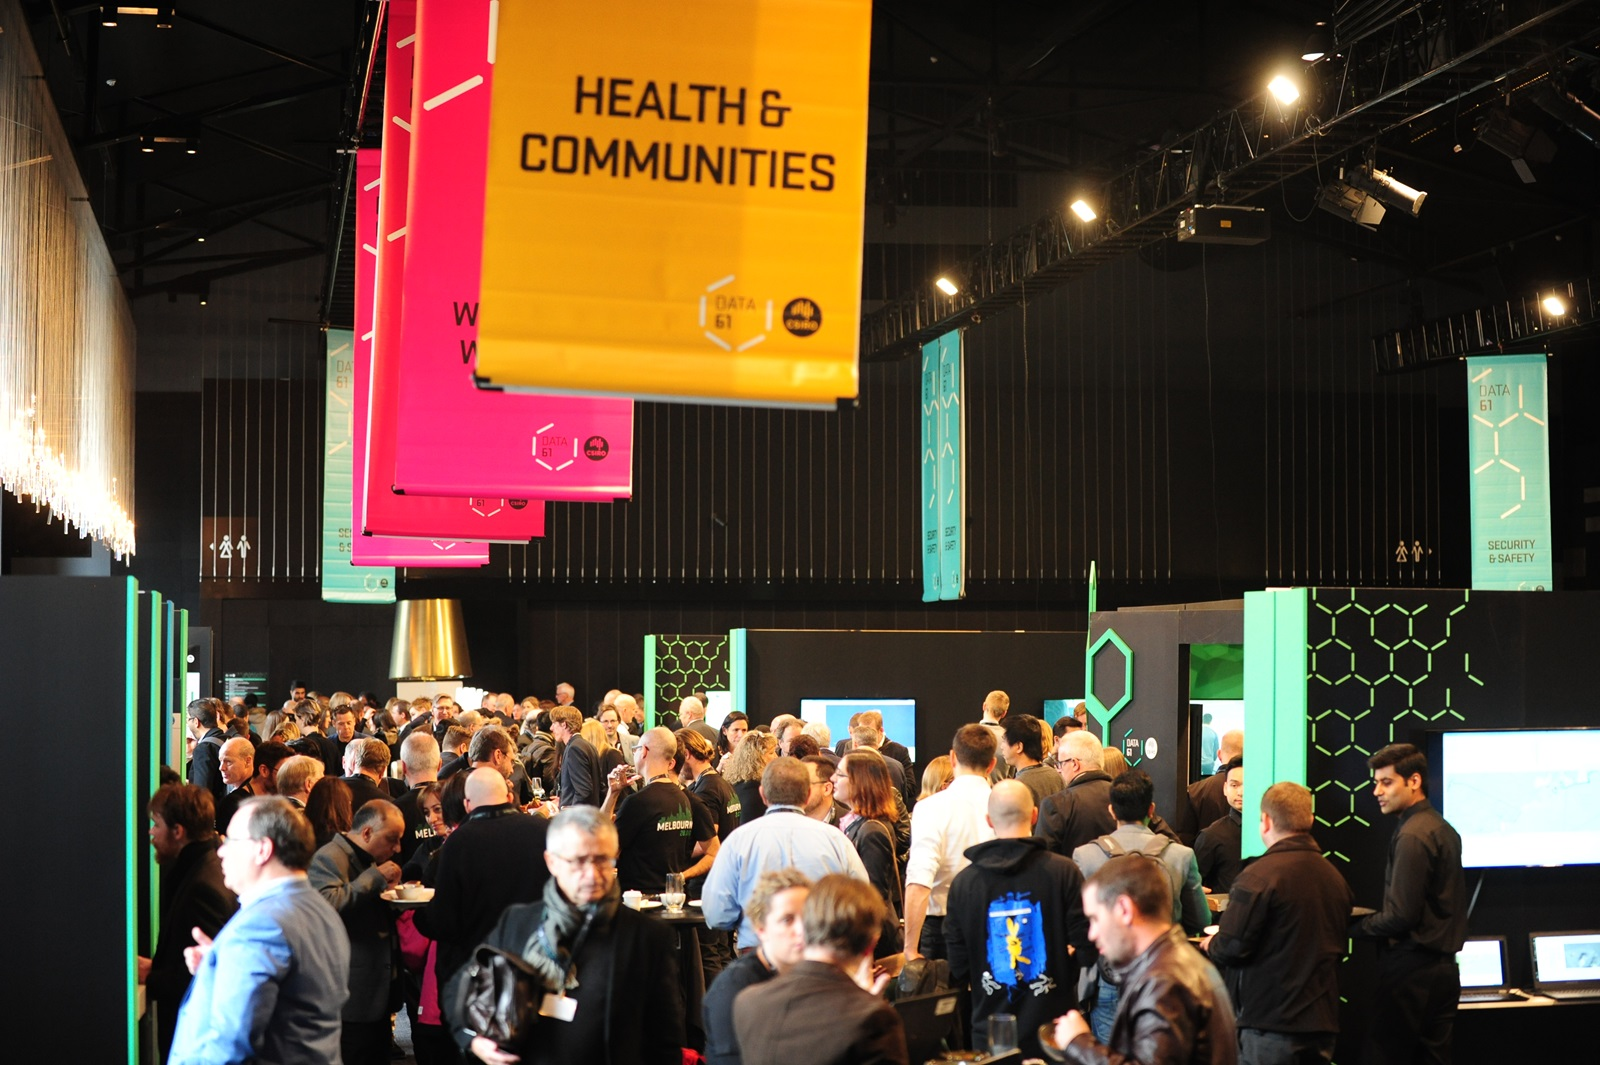
\includegraphics
        [height=5cm]
        {figures/data61_live_2.jpg}
    \caption{DATA61 LIVE Event}\vspace{-4mm}
\end{figure}

\newpage
\section{Conclusion}
%!TEX root = ./intern_report.tex

\paragraph{}
I worked as a research intern at DATA61 for 24 weeks. During this time, I worked three intertwined projects under the supervision of Nicolas Hudson and Dr. Navinda Kottege. 

\paragraph{}
The first project was developing indoor-Trailnet: a classification based approach to the autonomous navigation problem. For this, first I built a robot with Uvindu Perera for data collection and testing. We designed the power distribution system of the robot and assembled a high level and low level controllers. We calculated the torque requirements for the motors, current, voltage and power limitations for the power supply components and motor controllers during this process. We learnt a lot through debugging the errors we came across and extensively troubleshooting whenever a component or circuit board is damaged to provide a report on the event. I also debugged the driver software for the motor controller and modified parts of it to fix certain issues since it was not being maintained anymore.

\begin{figure}[H]
    \centering
    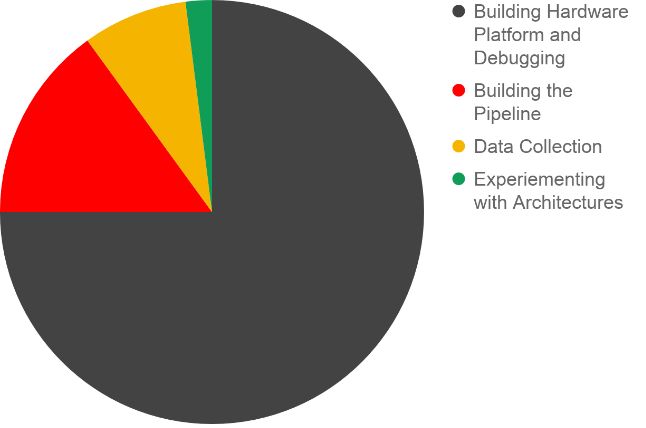
\includegraphics
        [width=9cm]
        {figures/time.PNG}
    \caption{Overview of our Time Spent}\vspace{-4mm}
\end{figure}

\paragraph{}
I learnt tensorflow and tensorflow-keras for this project and built a 20 layer residual network from scratch and trained it on the supercomputer cluster. Then I learnt tensorRT and deployed the trained network on Jetson TX2: a powerful embedded device that acted as the high level controller for the robot. I also learnt ROS (Robot Operating System) extensively, and created multiple ROS nodes and packages for testing, collecting data from sensors and for controlling the robot. 

\paragraph{}
For the next project of building an end to end pipeline for machine learning in robotics, I experimented and figured out the best practices when training models using large datasets on the supercomputer. I documented these experiments and the results, and proposed an efficient method to set up a writing and reading pipeline. I presented ~\cite{presentation} my pipeline in the Robotics Reading Group meeting. Many scientists were interested and some followed up via email asking questions and requesting to build tools for visualizing datasets.

\paragraph{}
The final project was experimental, where I explored different configurations of neural network architectures to build a robot that can climb hills while avoiding obstacles. Through literature survey and in-depth discussions with my supervisor, I learnt a lot about the structure of Deep Convolutional Neural Networks and possible methods of combining scaler data with the images to train a network. I tried several approaches here: solving the problem as a classification and a regression and using different ways to combine the inputs into the network. However, I was unable to get good results within the time we had there, due to the problems in data collection and the lack of time as we had to spend most of the time building and debugging the robot platform.

\paragraph{}
Also, I learnt about cross modal learning transfer and neural network distillation process through literature survey as a part of the project that was initially given, before we were changed into a different project a week later. Before and during the internship program, I expressed my interest in working in a project where I can develop algorithms and tackle abstract problems that could lead to new research and a publication. Unfortunately such a project was not available for interns at the time and my supervisors were satisfied with the work I was doing with hardware and deployment of machine learning. However, I learnt a lot through these projects and it had been a great experience. I also got familiarized with the software tools widely used in academia, high end sensors and controllers, and I daily worked with the Bracewell cluster, which is one of the world's largest supercomputer clusters. 

\paragraph{}
In addition to that, I learnt the etiquettes and responsibilities of working as an employee in a company. Helping others and asking for help, attending meetings and following up via official emails, documenting all the tasks and weekly progress in the wiki pages of CSIRO helped me learn a lot about these responsibilities. The work culture in DATA61 is exceptionally inclusive, where we got to work with people of multiple nationalities and share our culture. The students are allowed to work on their own pace and I was allowed to work overnight on multiple days and work on weekends as well. I also got to attend events such as DATA61 LIVE, where I could attend to many talks and discussion forums and observe the development of cutting edge technology of Australia through the exhibits.

\paragraph{}
From my experience, I would suggest DATA61 to assess the skills of the interns and assign them to projects relevant to those skills, to utilize their full potential for a project. Also, it would help if they can give an overview of the project at the beginning of the internship and set incremental goals to be completed at given deadlines. I found it disorienting when the project given to me before the internship was changed as I reached there and changed again a week later to settle on an experimental project of my supervisor that subsequently evolved into the three above projects (that I explained in Chapter 2) through the period of six months. 

\paragraph{}
I would also like to suggest NAITA to computerize the supervision process, where interns can submit the intern diary and monthly reports online. This would help because in organizations like CSIRO, the students are expected to maintain an online diary and the interns can save time by writing by hand the same thing they have typed into the online diary.

\paragraph{}
Therefore, I can conclude that my overall experience in DATA61 was great. I had the opportunity to learn a lot and make contacts. I am deeply thankful to the Industrial Training Division of our university and NAITA for this internship and I am thankful for DATA61 and my supervisors for providing me with such an exceptional opportunity and a training experience.







\newpage



\bibliographystyle{abbrv} 
\bibliography{biblo}
\end{document}